% ============================================================
%  main.tex — FORMATO ACADÉMICO BASADO EN IEEE (dos columnas)
%  Informe EVI. 6 — Auditoría socioambiental de la Mina Marlin
%  (Montana Exploradora de Guatemala, S.A. / Goldcorp), San Marcos, Guatemala
%  UNAP-FIM | Escuela Profesional de Ingeniería de Minas
%
%  Compilar con: pdflatex -> biber -> pdflatex -> pdflatex
%  (o simplemente: latexmk -pdf main.tex)
%
%  ATENCIÓN AL GRUPO: este archivo y config/preambulo.tex los toca UNA
%  SOLA PERSONA. Cada integrante edita únicamente su archivo de secciones/.
%
%  JERARQUÍA DE TÍTULOS EN LOS ARCHIVOS DE secciones/:
%     \chapter{}       -> capítulo      (nivel 1, centrado y grande)
%     \section{}       -> sección       (nivel 2, negrita)
%     \subsection{}    -> subsección    (nivel 3, cursiva)
%     \subsubsection{} -> sub-subsec.   (nivel 4, cursiva en línea)
% ============================================================

\documentclass[journal,onecolumn,10pt,a4paper]{IEEEtran}

% --- Configuración (no editar sin avisar al grupo) -------------------
% =====================================================================
%  PREÁMBULO — paquetes y configuración global
%  El \documentclass va en main.tex, NO aquí.
%  Stack probado en Overleaf: compilador pdfLaTeX + motor Biber.
% =====================================================================

% --- Codificación de entrada y de fuente -----------------------------
% utf8 permite escribir acentos y ñ directamente en los .tex.
% T1 evita que las palabras con acento se partan mal al final de línea.
\usepackage[utf8]{inputenc}
\usepackage[T1]{fontenc}

% --- Tipografía: Times New Roman -------------------------------------
% mathptmx sustituye la fuente por Times (requisito típico de informes
% universitarios). Si la universidad exige ARIAL, hay que cambiar el
% compilador a XeLaTeX y usar fontspec con \setmainfont{Arial}.
\usepackage{mathptmx}

% --- Márgenes --------------------------------------------------------
% 3 cm a la izquierda (para el anillado/empastado), 2,5 cm el resto.
\usepackage[a4paper,left=3cm,right=2.5cm,top=2.5cm,bottom=2.5cm]{geometry}

% --- Idioma español --------------------------------------------------
% es-tabla        -> los flotantes se rotulan «Tabla», no «Cuadro».
% es-nodecimaldot -> no fuerza la coma decimal en modo matemático.
% es-lcroman      -> numera los preliminares en romanos MINÚSCULOS (i, ii,
%                    iii), que es la convención académica. Sin esta opción,
%                    babel-spanish los pone en mayúsculas (I, II, III).
\usepackage[spanish,es-tabla,es-nodecimaldot,es-lcroman]{babel}

% --- Interlineado ----------------------------------------------------
% ÚNICO lugar donde se controla el interlineado de todo el documento.
% \onehalfspacing = 1,5 líneas (el que estamos usando).
% Si el docente pidiera interlineado doble, cambia a \doublespacing.
% Si necesitas comprimir para entrar en un límite de páginas, \singlespacing.
\usepackage{setspace}
\onehalfspacing

% --- Imágenes --------------------------------------------------------
% graphicspath evita tener que escribir la ruta completa en \includegraphics:
% basta con \includegraphics{mapa_ubicacion.png}.
\usepackage{graphicx}
\graphicspath{{imagenes/}{imagenes/mapas/}{imagenes/diagramas/}{imagenes/fotos/}{imagenes/logos/}}

% --- Tablas ----------------------------------------------------------
% booktabs  -> líneas horizontales de calidad (\toprule, \midrule, \bottomrule).
% longtable -> tablas que se parten en varias páginas (la matriz de no
%              conformidades del Anexo B seguro la necesita).
% tabularx  -> columnas de ancho automático que ajustan al ancho de página.
% multirow  -> celdas que ocupan varias filas.
% array     -> tipos de columna personalizados (ver config/comandos.tex).
\usepackage{booktabs}
\usepackage{longtable}
\usepackage{tabularx}
\usepackage{multirow}
\usepackage{array}

% --- Leyendas de tablas y figuras ------------------------------------
% Norma APA / uso académico: el rótulo de la TABLA va ARRIBA y el de la
% FIGURA va ABAJO. Aquí se fija ese comportamiento para todo el documento.
\usepackage{caption}
\captionsetup[table]{position=top,labelsep=period,font=small,labelfont=bf}
\captionsetup[figure]{position=bottom,labelsep=period,font=small,labelfont=bf}

% --- Listas ----------------------------------------------------------
% enumitem permite controlar sangrías y separación de itemize/enumerate.
\usepackage{enumitem}
\setlist{itemsep=2pt,parsep=0pt,topsep=4pt}

% --- Posicionamiento de flotantes ------------------------------------
% float habilita el especificador [H] = «aquí exactamente, sin discutir».
\usepackage{float}

% --- Páginas apaisadas -----------------------------------------------
% pdflscape gira una página completa en el PDF. Imprescindible para la
% Tabla 3 (matriz de no conformidades) y la Tabla 4 (plan de acción).
\usepackage{pdflscape}

% --- Color (necesario para los enlaces de hyperref) ------------------
\usepackage{xcolor}
\definecolor{azuloscuro}{RGB}{0,51,102}

% =====================================================================
%  BIBLIOGRAFÍA — biblatex en estilo APA 7 con motor Biber
% =====================================================================
% csquotes es OBLIGATORIO antes de biblatex (gestiona las comillas).
\usepackage{csquotes}
\usepackage[backend=biber,style=apa,sortlocale=es_ES,natbib=true]{biblatex}
% Traduce al español los elementos fijos de las citas («y», «et al.», «s. f.»).
\DeclareLanguageMapping{spanish}{spanish-apa}
% Archivo con TODAS las referencias del informe.
\addbibresource{referencias.bib}

% =====================================================================
%  HYPERREF — SIEMPRE EL ÚLTIMO PAQUETE EN CARGARSE
% =====================================================================
% Convierte en enlaces clicables el índice, las referencias cruzadas y
% las URLs, y genera los marcadores (bookmarks) del PDF.
\usepackage[
  colorlinks=true,
  linkcolor=azuloscuro,     % enlaces internos (índice, \ref)
  citecolor=azuloscuro,     % citas bibliográficas
  urlcolor=azuloscuro,      % URLs externas
  bookmarks=true,
  bookmarksnumbered=true,
  breaklinks=true,
  % plainpages=false hace que las anclas del PDF usen el número de página tal
  % como se imprime (i, ii, 1, 2...). Junto con el \pagenumbering{roman} que
  % main.tex activa desde la portada, evita anclas duplicadas.
  plainpages=false,
  pdftitle={Auditoría socioambiental de la Mina Marlin — Informe EVI. 6},
  pdfsubject={Auditoría ambiental},
  pdfkeywords={auditoría socioambiental, Mina Marlin, Goldcorp, ISO 14001, ISO 19011, PHVA}
]{hyperref}
% Rompe las URLs largas de la bibliografía para que no se salgan del margen.
\usepackage{url}
\urlstyle{same}

% ============================================================
%  DATOS DE PORTADA (bloque de título estilo IEEE)
%
%  Ya NO es una carátula a página completa: IEEEtran compone el
%  título, los autores y la afiliación en la cabecera de la primera
%  página, y el resumen va justo debajo.
%
%  RELLENA lo que está entre llaves { }:
%    - el nombre del curso
%    - el nombre del docente
%  Y VERIFICA LA LISTA DE INTEGRANTES (ver nota más abajo).
% ============================================================

\title{\LARGE\bfseries Auditoría Socioambiental de la Mina Marlin\\
       (Montana Exploradora de Guatemala, S.\,A. / Goldcorp):\\
       Análisis del Proceso de Auditoría y Propuesta de\\
       Plan de Mejora Continua bajo el Ciclo PHVA}

% ------------------------------------------------------------
%  INTEGRANTES
%  VERIFICAR: esta lista se tomó del trabajo de Perforación y Voladura,
%  asumiendo que el grupo es el mismo. Si el grupo de este curso es
%  distinto, corrige los nombres aquí. La bitácora preveía un grupo de
%  4 o 5 integrantes; aquí hay 4.
% ------------------------------------------------------------
\author{%
  \IEEEauthorblockN{%
    \textbf{Brandon Gabriel Quispe Tapia}\IEEEauthorrefmark{1},
    \textbf{Cristian Ivan Huanca Constancia}\IEEEauthorrefmark{1},\\
    \textbf{Rudy Javier Mollocondo Mollocondo}\IEEEauthorrefmark{1} y
    \textbf{Britt Lizardo Gemio Mamani}\IEEEauthorrefmark{1}%
  }\\[4pt]
  \IEEEauthorblockA{\IEEEauthorrefmark{1}Escuela Profesional de Ingeniería de Minas,
                    Facultad de Ingeniería de Minas\\
                    Universidad Nacional del Altiplano, Puno, Perú\\
                    \textit{Curso: {NOMBRE DEL CURSO} --- Evidencia N.\textsuperscript{o} 6}\\
                    \textbf{Docente:} {Grado y nombre completo del docente}}%
  \thanks{Manuscrito elaborado en 2026. Trabajo desarrollado a partir de la
  \textit{Human Rights Assessment of Goldcorp's Marlin Mine}, evaluación
  socioambiental independiente realizada por On Common Ground Consultants Inc.
  (2010) sobre la operación de Montana Exploradora de Guatemala, S.\,A.,
  departamento de San Marcos, Guatemala.}}

\markboth{Universidad Nacional del Altiplano --- Auditoría Ambiental, 2026}%
         {Auditoría Socioambiental de la Mina Marlin}

% =====================================================================
%  COMANDOS Y ATAJOS PROPIOS DEL INFORME
%  Objetivo: escribir siempre igual los nombres largos y las unidades,
%  para que el documento quede uniforme aunque lo redacten 5 personas.
% =====================================================================

% --- Tipos de columna para tablas ------------------------------------
% L{3cm} = columna de ancho fijo alineada a la izquierda con salto de línea
% C{3cm} = ídem centrada       R{3cm} = ídem alineada a la derecha
% Se usan sobre todo en la matriz de no conformidades (Tabla 3).
\newcolumntype{L}[1]{>{\raggedright\arraybackslash}p{#1}}
\newcolumntype{C}[1]{>{\centering\arraybackslash}p{#1}}
\newcolumntype{R}[1]{>{\raggedleft\arraybackslash}p{#1}}
% Y = como X de tabularx pero con el texto sin justificar (evita huecos feos)
\newcolumntype{Y}{>{\raggedright\arraybackslash}X}

% --- Nombres recurrentes ---------------------------------------------
% Escribe \mina en lugar de teclear el nombre completo cada vez.
\newcommand{\mina}{Mina Marlin}
\newcommand{\titular}{Montana Exploradora de Guatemala, S.\,A.}
\newcommand{\auditora}{On Common Ground Consultants Inc.}
\newcommand{\hria}{\textit{Human Rights Assessment of Goldcorp's Marlin Mine}}

% --- Unidades y notación técnica -------------------------------------
% Evita que se escriba «g/t» de tres formas distintas en el mismo informe.
\newcommand{\gt}{g/t}                        % ley: gramos por tonelada
\newcommand{\ozAu}{oz Au}                    % onzas de oro
\newcommand{\ozAg}{oz Ag}                    % onzas de plata
\newcommand{\msnm}{m\,s.\,n.\,m.}            % metros sobre el nivel del mar
\newcommand{\tdia}{t/día}                    % toneladas por día

% --- Clasificación de hallazgos (ISO 19011) --------------------------
% Úsalos en la columna «Clasificación» de la matriz de no conformidades
% para que las tres categorías se vean siempre igual.
\newcommand{\NCmayor}{\textbf{NC mayor}}
\newcommand{\NCmenor}{NC menor}
\newcommand{\OBS}{Observación}

% --- Marcador de pendiente -------------------------------------------
% \pendiente{texto} imprime una nota visible en el PDF mientras se redacta.
% CUANDO EL INFORME ESTÉ TERMINADO: comenta la primera definición y
% descomenta la segunda para que los pendientes desaparezcan del PDF final.
\newcommand{\pendiente}[1]{\textcolor{red}{\small[PENDIENTE: #1]}}
%\renewcommand{\pendiente}[1]{}

% --- Cita textual destacada ------------------------------------------
% APA: las citas de más de 40 palabras van en bloque, sin comillas y
% con sangría. \citalarga{texto}{referencia} lo hace automáticamente.
\newenvironment{citalarga}
  {\begin{quote}\singlespacing\small}
  {\end{quote}\normalsize}


\begin{document}

\maketitle

% ------------------------------------------------------------
%  RESUMEN + PALABRAS CLAVE (a una columna)
% ------------------------------------------------------------
% =====================================================================
%  RESUMEN Y PALABRAS CLAVE
%  Responsable: TODOS (se redacta AL FINAL, cuando el informe esté cerrado)
%  Extensión objetivo: 250 a 300 palabras
%
%  En este formato el resumen NO es un capítulo numerado: va en el entorno
%  abstract de IEEEtran, justo debajo del bloque de autores y a una sola
%  columna. No lleva \chapter ni \section.
% =====================================================================

\begin{abstract}
% TODO: Un solo párrafo compacto que responda, en este orden:
%   1) Qué caso se analiza  -> Mina Marlin, Montana Exploradora / Goldcorp,
%      municipios de San Miguel Ixtahuacán y Sipacapa, San Marcos, Guatemala;
%      oro y plata; operó de 2005 a 2017.
%   2) Qué auditoría se estudia -> la Human Rights Assessment of Goldcorp's
%      Marlin Mine, de On Common Ground Consultants (2010), evaluación
%      socioambiental independiente de más de 200 páginas.
%   3) Qué metodología se aplicó en ESTE informe -> revisión documental de
%      fuentes primarias, análisis bajo ISO 19011:2018 y clasificación de
%      hallazgos en no conformidades.
%   4) Hallazgos centrales -> los siete ejes; en especial la ausencia de
%      consulta previa (Convenio 169 de la OIT), los riesgos de drenaje
%      ácido de roca y calidad de agua, la seguridad privada armada y la
%      debilidad de los mecanismos de queja.
%   5) El resultado propuesto -> plan de mejora continua bajo el ciclo PHVA
%      alineado a los IFC Performance Standards, el GISTM e IRMA.
%
% REGLA: el resumen NO lleva citas, ni tablas, ni figuras. Solo prosa.

\pendiente{redactar el resumen (250--300 palabras)}
\end{abstract}

\begin{IEEEkeywords}
% TODO: de 4 a 6 palabras clave separadas por punto y coma.
% Sugeridas: auditoría socioambiental; Mina Marlin; ISO 19011; ciclo PHVA;
% derechos humanos; no conformidad.
\pendiente{4 a 6 palabras clave}
\end{IEEEkeywords}
          % Todos (se redacta al final)

% ------------------------------------------------------------
%  ÍNDICES (a una columna, justo después del resumen)
%  tocdepth=2 -> el índice llega hasta el nivel "Sección" y no baja
%  a subsección, para que quede corto y limpio.
% ------------------------------------------------------------
\setcounter{tocdepth}{2}
\tableofcontents

% Los índices de figuras y tablas los pedía la estructura del curso.
% Si el docente no los exige, comenta estas dos líneas.
\listoffigures
\listoftables

% ------------------------------------------------------------
%  A PARTIR DE AQUÍ, DOS COLUMNAS
% ------------------------------------------------------------
\twocolumn

% =====================================================================
%  1. INTRODUCCIÓN
%  Responsable: TODOS
%  ESTADO: REDACTADO (1 de agosto de 2026) — ~950 palabras
%  Se redactó AL FINAL, con el informe ya cerrado, para que el último
%  párrafo describa la estructura real y no la prevista.
% =====================================================================

\section{Introducción}
\label{sec:introduccion}

La minería es una actividad de alto impacto socioambiental por definición y no por
defecto de gestión. Transforma de manera irreversible el relieve, moviliza
volúmenes de material que superan en órdenes de magnitud a los del mineral
aprovechado, consume y puede alterar la calidad del agua de las cuencas donde se
emplaza, y se implanta sobre territorios que rara vez la solicitaron. Su
particularidad frente a otras actividades industriales reside en que no puede
elegir su localización: se instala donde está el yacimiento, y con frecuencia el
yacimiento está bajo el territorio de poblaciones rurales o indígenas cuya
economía depende directamente de la tierra y del agua que la operación va a
utilizar. De esa condición estructural nace la doble dimensión —ambiental y
social— que da nombre a este informe y que ningún instrumento de control puede
abordar por separado sin quedar ciego ante la mitad del problema.

Frente a ese impacto, la auditoría opera como herramienta de verificación. No
previene, como el estudio de impacto ambiental, ni sanciona, como la fiscalización
estatal: comprueba, mediante un proceso sistemático, documentado e independiente,
si la conducta efectiva de la organización se ajusta a criterios previamente
establecidos, y traduce las desviaciones detectadas en hallazgos y recomendaciones
\parencite{iso2018iso19011}. Su valor depende por completo de tres condiciones
que este trabajo examina con detenimiento: que los criterios sean exigentes y
explícitos, que quien audita sea efectivamente independiente de quien es auditado,
y que exista alguien con capacidad y mandato para verificar que lo recomendado se
cumplió. Cuando alguna de las tres falla, el resultado puede ser un documento
técnicamente correcto y prácticamente inocuo.

El caso seleccionado para este análisis es la Mina Marlin, operada por Montana
Exploradora de Guatemala, S.\,A., filial de Goldcorp Inc., en el departamento de
San Marcos, Guatemala, entre 2005 y 2017. La elección responde a cuatro criterios.

El primero es la existencia de un documento de auditoría público, independiente y
exhaustivo: la \hria, elaborada por On Common Ground Consultants Inc. y publicada
en mayo de 2010, con más de doscientas páginas y versión bilingüe
\parencite{oncommonground2010hria}. El segundo, y decisivo, es que ese documento
es \textbf{ambiental y social a la vez}: evaluó siete ejes —consulta, ambiente,
trabajo, adquisición de tierras, inversión económica y social, seguridad y acceso
a remediación— aplicando estándares internacionales de derechos humanos, que es
exactamente el tipo de auditoría socioambiental que este trabajo debe analizar. El
tercero es la disponibilidad de datos técnicos verificables en fuentes primarias:
el informe técnico NI 43-101 presentado ante la Comisión de Bolsa y Valores de los
Estados Unidos \parencite{sec2011ni43101} y la documentación de la Corporación
Financiera Internacional \parencite{ifcsfmarlin}. El cuarto es que el caso tiene
\textbf{ciclo completo}: operación, conflicto, auditoría, plan de acción, cierre y
post-cierre. Ello permite evaluar la mejora continua sobre un expediente cerrado y
no sobre una operación en curso, y comprobar si las recomendaciones formuladas en
2010 llegaron efectivamente a cumplirse antes del cierre de 2017.

Se consideraron y descartaron otros casos. Brumadinho, Mount Polley y Samarco
disponen de investigaciones técnicas de calidad superior en materia geotécnica,
pero sus paneles de expertos son auditorías esencialmente técnicas: excelentes
para el eje ambiental y débiles para el social. Espinar, en el Perú, presenta un
componente social y de diálogo muy fuerte, pero su documento ancla es un monitoreo
sanitario ambiental participativo y no una auditoría en sentido estricto. Marlin
resultó ser el único caso en que el documento auditado combina de forma nativa
ambas dimensiones.

La pertinencia del caso para un lector peruano merece explicitarse, pese a
tratarse de una operación guatemalteca. La conflictividad socioambiental minera en
el Perú responde a una estructura semejante —operaciones de gran escala sobre
territorios de comunidades campesinas e indígenas, disputas sobre calidad y
disponibilidad de agua, y déficits de consulta previa—, de modo que el caso
funciona como término de comparación. Más aún: permite contrastar dos modelos de
control de naturaleza distinta, la auditoría voluntaria financiada por la empresa
auditada frente a la fiscalización estatal con potestad sancionadora que ejerce el
Organismo de Evaluación y Fiscalización Ambiental
\parencite{congreso2009ley29325}. Ese contraste, desarrollado en la sección
\ref{sec:critico}, constituye uno de los aportes centrales del trabajo.

El informe se organiza en diez secciones. Tras estos preliminares y el enunciado
de los objetivos, la sección \ref{sec:marco} construye el marco teórico y
normativo: delimita la auditoría ambiental frente a la fiscalización y a la
evaluación de impacto ambiental, expone las normas ISO 14001:2015 e
ISO 19011:2018 y los estándares internacionales de desempeño social, y presenta el
marco peruano de referencia y el ciclo PHVA. La sección \ref{sec:unidad} describe
la unidad minera: titularidad, ubicación, entorno social, geología, método de
explotación, procesamiento, producción e infraestructura crítica. La sección
\ref{sec:auditoria} reconstruye el proceso de auditoría —origen del encargo,
organismo auditor, equipo, alcance, criterios y metodología— y lo contrasta con
las fases que establece la ISO 19011:2018. La sección \ref{sec:hallazgos}
sistematiza los hallazgos en una matriz de no conformidades y desarrolla los
cuatro de mayor gravedad. La sección \ref{sec:critico} evalúa críticamente el
proceso: independencia, limitaciones metodológicas, conflicto de evidencia sobre
la contaminación, eficacia real y contraste con el régimen peruano. La sección
\ref{sec:plan} formula la propuesta de plan de mejora continua bajo el ciclo PHVA.
Las secciones \ref{sec:conclusiones} y \ref{sec:recomendaciones} recogen,
respectivamente, las conclusiones referidas a cada objetivo específico y las
recomendaciones dirigidas a la empresa, al Estado, a las comunidades y a la
comunidad académica. Cierran el documento las referencias y cinco anexos.
      % Todos (al final, en conjunto)
% =====================================================================
%  2. OBJETIVOS
%  Responsable: TODOS
%  ESTADO: REDACTADO (1 de agosto de 2026)
%
%  REGLA: cada objetivo específico tiene DESPUÉS su conclusión
%  correspondiente en la sección 9, en el mismo orden. Son pares.
%  Si añades un objetivo, añades una conclusión.
% =====================================================================

\section{Objetivos}
\label{sec:objetivos}

% ---------------------------------------------------------------------
\subsection{Objetivo general}

Analizar el proceso y los resultados de la auditoría socioambiental aplicada a la
Mina Marlin (Montana Exploradora de Guatemala, S.\,A. / Goldcorp), departamento de
San Marcos, Guatemala, con el fin de formular una propuesta de plan de mejora
continua fundamentada en el ciclo PHVA y en los estándares internacionales de
desempeño ambiental y social.

% ---------------------------------------------------------------------
\subsection{Objetivos específicos}

\begin{enumerate}
  \item Describir la unidad minera y su entorno físico, geológico y social,
        identificando los aspectos de la operación que determinan su perfil de
        riesgo socioambiental.
  \item Identificar el alcance, los criterios de auditoría y la metodología
        aplicados por el equipo auditor, y contrastarlos con las directrices de la
        ISO 19011:2018.
  \item Clasificar los hallazgos ambientales y sociales de la auditoría según las
        categorías de no conformidad mayor, no conformidad menor y observación,
        estableciendo para cada uno su evidencia objetiva, el criterio incumplido
        y su estado de cierre.
  \item Evaluar críticamente la independencia del proceso de auditoría, sus
        limitaciones metodológicas declaradas y su eficacia real sobre la conducta
        de la organización auditada.
  \item Proponer un plan de mejora continua estructurado sobre el ciclo PHVA, con
        acciones verificables mapeadas a requisitos concretos de los IFC
        Performance Standards, el GISTM y el estándar IRMA.
\end{enumerate}
         % Todos (al final, en conjunto)
% =====================================================================
%  3. MARCO TEÓRICO Y NORMATIVO
%  Responsable: INTEGRANTE 1
%  Extensión objetivo: 6 a 8 páginas — aprox. 2.600 a 3.000 palabras
%  Fuente principal: Sección D de docs/bitacora_decisiones.md
%
%  ADVERTENCIA: esta sección se llena de definiciones y es fácil que quede
%  como un copiar-pegar de normas. Para evitarlo, cierra CADA subsección
%  con una frase que la conecte con el caso Marlin.
% =====================================================================

\section{Marco teórico y normativo}

% TODO (párrafo de entrada, ~80 palabras): anuncia los tres bloques de esta
%   sección: (a) qué es una auditoría ambiental y en qué se diferencia de
%   figuras vecinas; (b) los estándares internacionales aplicables; y (c) el
%   marco peruano de referencia que servirá para el contraste de la sección 7.

% ---------------------------------------------------------------------
\subsection{La auditoría ambiental: definición, tipos y delimitación conceptual}
% Extensión: ~1,5 páginas / 550 palabras

% TODO: Definir auditoría ambiental como proceso SISTEMÁTICO, DOCUMENTADO
%   e INDEPENDIENTE para obtener evidencia objetiva y evaluarla de manera
%   objetiva frente a criterios de auditoría. Subrayar las tres palabras.
%   Fuente: \cite{iso2018iso19011}

% TODO: Tipología por quién audita:
%   - Primera parte (interna): la propia organización se audita.
%   - Segunda parte (externa de proveedor/cliente): audita una parte interesada.
%   - Tercera parte (certificación): organismo independiente acreditado.
%   PREGUNTA CLAVE PARA EL INFORME: ¿de qué tipo fue la HRIA de Marlin?
%   Fue externa e independiente en su ejecución, pero financiada por la
%   empresa auditada. Anticipa aquí en una frase esa tensión y remite a la
%   sección 7. Fuente: \cite{oncommonground2010hria}

% TODO: Tipología por objeto: de sistema de gestión, de cumplimiento legal,
%   de residuos, energética, sectorial vs. integrada.

% TODO: DELIMITACIÓN CONCEPTUAL (este párrafo suele valer varios puntos):
%   - Auditoría   = verificación de conformidad frente a criterios; no sanciona.
%   - Fiscalización / supervisión = potestad ESTATAL de control y sanción
%     (en Perú, el OEFA). Fuente: \cite{congreso2009ley29325}
%   - EIA = instrumento PREDICTIVO y EX ANTE, previo a la operación.
%     Fuente: \cite{congreso2001ley27446}
%   Recomendación: cierra con una tabla comparativa de tres columnas
%   (auditoría / fiscalización / EIA) por filas: quién lo hace, cuándo,
%   carácter vinculante, consecuencia jurídica.

% --- Tabla comparativa (opcional pero muy recomendable) ---------------
%\begin{table}[H]
%  \centering
%  \caption{Diferencias entre auditoría ambiental, fiscalización y evaluación de impacto ambiental}
%  \label{tab:auditoria-vs-fiscalizacion}
%  \begin{tabularx}{\textwidth}{@{}l Y Y Y@{}}
%    \toprule
%    \textbf{Criterio} & \textbf{Auditoría} & \textbf{Fiscalización} & \textbf{EIA} \\
%    \midrule
%    Quién la realiza &  &  &  \\
%    Momento          &  &  &  \\
%    Carácter         &  &  &  \\
%    Consecuencia     &  &  &  \\
%    \bottomrule
%  \end{tabularx}
%  \footnotesize Nota. Elaboración propia a partir de \textcite{iso2018iso19011} y \textcite{congreso2009ley29325}.
%\end{table}

% ---------------------------------------------------------------------
\subsection{ISO 14001:2015 y el sistema de gestión ambiental}
% Extensión: ~1 página / 380 palabras

% TODO: Norma certificable; Estructura de Alto Nivel (Anexo SL) que la hace
%   compatible con ISO 9001 e ISO 45001. Explicar contexto de la
%   organización, liderazgo, planificación, apoyo, operación, evaluación del
%   desempeño y mejora. Señalar que la norma se ORGANIZA sobre el ciclo PHVA,
%   lo que enlaza directamente con la sección 8 de este informe.
%   Fuente: \cite{iso2015iso14001}

% TODO: Concepto de aspecto ambiental vs. impacto ambiental, con un ejemplo
%   tomado del propio caso (aspecto: uso de cianuro en la lixiviación CIL;
%   impacto potencial: contaminación de agua superficial y subterránea).

% ---------------------------------------------------------------------
\subsection{ISO 19011:2018 y la conducción de la auditoría}
% Extensión: ~1,5 páginas / 550 palabras

% TODO: Directrices para auditar sistemas de gestión. Desarrollar:
%   - Los principios: integridad, presentación imparcial, debido cuidado
%     profesional, confidencialidad, independencia, enfoque basado en la
%     evidencia y enfoque basado en riesgos.
%   - Gestión del programa de auditoría.
%   - FASES: inicio -> revisión documental -> preparación del plan ->
%     actividades in situ (reunión de apertura, recolección de evidencia por
%     entrevista, muestreo y observación, reunión de cierre) -> informe ->
%     seguimiento.
%   - Competencia y evaluación de los auditores.
%   Fuente: \cite{iso2018iso19011}

% TODO: DEFINICIONES QUE SE USARÁN EN LA SECCIÓN 6 (déjalas explícitas aquí,
%   porque de ellas depende la clasificación de la matriz de hallazgos):
%   criterio de auditoría, evidencia objetiva, hallazgo, conformidad,
%   NO CONFORMIDAD MAYOR, NO CONFORMIDAD MENOR, OBSERVACIÓN, conclusión de
%   auditoría, acción correctiva y acción preventiva.

% ---------------------------------------------------------------------
\subsection{Estándares internacionales de desempeño ambiental y social}
% Extensión: ~2 páginas / 750 palabras

\subsubsection{IFC Performance Standards}
% TODO: PS1 (evaluación y gestión de riesgos e impactos), PS4 (salud y
%   seguridad de la comunidad), PS5 (adquisición de tierras y reasentamiento
%   involuntario), PS7 (pueblos indígenas, incluye el consentimiento libre,
%   previo e informado) y PS8 (patrimonio cultural).
%   IMPORTANTE: explica por qué son directamente exigibles en este caso —
%   la IFC financió el proyecto con un préstamo de US$ 45 millones, lo que
%   activó sus políticas de salvaguarda. Fuentes: \cite{ifcsfmarlin}, \cite{cao2006marlin}

\subsubsection{Convenio 169 de la OIT y la consulta previa}
% TODO: Obligación de consulta previa, libre e informada a pueblos indígenas
%   y tribales. Es el criterio incumplido más importante de todo el caso.
%   Fuente: \cite{oit1989convenio169}

\subsubsection{Voluntary Principles on Security and Human Rights}
% TODO: Marco para empresas extractivas sobre uso de seguridad privada y
%   pública. Se recomendó su adopción justamente por el eje de seguridad
%   de la auditoría. Fuente: \cite{vpshr2000principios}

\subsubsection{ICMM, GISTM e IRMA}
% TODO: - ICMM Mining Principles. Fuente: \cite{icmmsfprincipios}
%       - GISTM (2020): desarrollado por ICMM, UNEP y PRI DESPUÉS de
%         Brumadinho; seis áreas temáticas, 15 principios y 77 requisitos
%         auditables; su Tema I exige debida diligencia en derechos humanos
%         y participación de las personas afectadas.
%         Fuentes: \cite{icmm2020gistm}, \cite{unep2020gistm}
%       - IRMA: más de 420 requisitos auditables, auditoría independiente de
%         tercera parte, y exigencia de al menos 90 % de cumplimiento en cada
%         una de las cuatro áreas de principios para certificar.
%         Fuente: \cite{irmasfstandard}

% ---------------------------------------------------------------------
\subsection{Marco normativo peruano de referencia}
% Extensión: ~1,5 páginas / 550 palabras
% NOTA: esta subsección NO se aplica al caso guatemalteco. Sirve para el
% contraste de la sección 7.5. Dilo explícitamente para que no parezca error.

% TODO: - Ley 28611, Ley General del Ambiente. \cite{congreso2005ley28611}
%       - Ley 27446, Ley del SEIA, y su reglamento D.S. 019-2009-MINAM;
%         rol del SENACE en la aprobación de EIA detallados.
%         \cite{congreso2001ley27446}, \cite{minam2009ds019}
%       - Ley 29325, SINEFA: el OEFA como ente rector de la fiscalización,
%         supervisión, evaluación, control y sanción ambiental de la mediana
%         y gran minería. \cite{congreso2009ley29325}
%       - D.S. 040-2014-EM, Reglamento de Protección y Gestión Ambiental
%         Minera; medidas correctivas del artículo 39. \cite{minem2014ds040}
%       - D.S. 042-2003-EM, compromiso previo y relación con comunidades.
%         \cite{minem2003ds042}
%       - Ley 29785, Ley de Consulta Previa. \cite{congreso2011ley29785}
%       - Mención de OSINERGMIN (seguridad de infraestructura), SUNAFIL
%         (seguridad y salud en el trabajo) y de la figura histórica del PAMA.

% ---------------------------------------------------------------------
\subsection{El ciclo PHVA como base de la mejora continua}
% Extensión: ~0,5 página / 200 palabras

% TODO: Planificar - Hacer - Verificar - Actuar, aplicado a la gestión
%   ambiental y social minera. Explicar brevemente cada fase porque la
%   sección 8 se construye enteramente sobre esta estructura:
%   - Planificar: política, aspectos e impactos, objetivos y metas.
%   - Hacer: controles operacionales, competencias, comunicación.
%   - Verificar: monitoreo, medición, auditoría interna, monitoreo
%     participativo (modelos AMAC en Marlin y mesa de diálogo en Espinar).
%   - Actuar: acciones correctivas, revisión por la dirección, cierre de
%     no conformidades.
%   Fuente: \cite{iso2015iso14001}

\pendiente{desarrollar la sección 3 (6--8 páginas)}
     % Integrante 1
% =====================================================================
%  4. DESCRIPCIÓN DE LA UNIDAD MINERA
%  Responsable: INTEGRANTE 2
%  ESTADO: REDACTADO (1 de agosto de 2026) — ~3.900 palabras
%  Fuente principal: Sección B de docs/bitacora_decisiones.md
%
%  Contiene la Tabla de reservas y leyes y la Tabla de capacidad de
%  tratamiento. Faltan por insertar la Figura 1 (mapa de ubicación) y la
%  Figura 2 (diagrama de flujo del proceso): los entornos están listos y
%  comentados, solo hay que colocar los archivos en imagenes/.
%
%  ############ LAS CUATRO ADVERTENCIAS DE DATOS ESTÁN RESUELTAS ##########
%  1) Capacidad de planta -> presentada como rango con su fuente en la
%     sección 4.7 y en su tabla, NO como cifra única.
%  2) Las ~24.282 t/día del NI 43-101 -> declaradas expresamente como
%     material total minado (mineral + desmonte), no capacidad de planta.
%  3) Mina Constancia (Perú) -> no se ha tomado ningún dato de esa
%     operación. Si alguien añade cifras nuevas, verificar la fuente.
%  4) Presa de relaves -> tipo, altura y volumen NO verificados en fuente
%     primaria de Marlin; se consigna como limitación de información en
%     la sección 4.9. NO rellenar esos datos sin el EIA detallado o el
%     informe de diseño de Knight Piésold.
%  ######################################################################
% =====================================================================

\section{Descripción de la unidad minera}
\label{sec:unidad}

La caracterización de la unidad minera no es un trámite descriptivo previo al
análisis de la auditoría, sino parte del análisis mismo. Los hallazgos que se
examinan en la sección \ref{sec:hallazgos} solo resultan inteligibles si antes se
comprende qué se extraía, con qué método, mediante qué procesos químicos, sobre
qué territorio y en convivencia con qué población. El uso de cianuro explica la
preocupación por la calidad del agua; el método mixto de explotación explica las
denuncias por agrietamiento de viviendas; la condición indígena del territorio
explica la exigencia de consulta previa; y la magnitud económica de la operación
explica tanto la intensidad del conflicto como la presión internacional que
terminó desembocando en la propia auditoría. Esta sección aporta, por tanto, las
premisas fácticas del resto del informe.

% ---------------------------------------------------------------------
\subsection{Identificación y evolución de la titularidad}

La operación analizada corresponde a la Mina Marlin, también denominada Proyecto
Marlin en la documentación técnica y financiera. Su titular directo fue
\titular, sociedad guatemalteca constituida el 6 de agosto de 1996. La matriz
corporativa durante la mayor parte de la vida útil fue Goldcorp Inc., empresa con
sede en Vancouver, Canadá; tras la fusión societaria de 2019, los activos
históricos de Goldcorp pasaron a integrarse en Newmont
\parencite{sec2011ni43101, goldcorp2023marlin}.

La cadena de titularidad tiene relevancia auditora directa, porque las
obligaciones asumidas en una etapa fueron heredadas por operadores distintos de
quienes las contrajeron. El yacimiento fue descubierto en 1998 por Montana
Exploradora. En 2000 la propiedad fue adquirida por Francisco Gold, compañía que
en 2002 se fusionó con Glamis Gold. Fue Glamis quien obtuvo del Ministerio de
Energía y Minas de Guatemala la licencia de explotación, otorgada el 27 de
noviembre de 2003, y quien gestionó el financiamiento internacional del proyecto.
La construcción se desarrolló entre 2004 y 2005, y la producción de oro y plata
se inició hacia finales de 2005. En 2006 Goldcorp adquirió Glamis Gold e incorporó
la operación a su portafolio. La producción cesó definitivamente el 31 de mayo de
2017 \parencite{sec2011ni43101, prensalibre2017cierre, goldcorp2023marlin}.

Un elemento decisivo de esta etapa inicial es el financiamiento. La Corporación
Financiera Internacional otorgó al proyecto un préstamo de US\$ 45 millones,
decisión que activó la aplicación de sus políticas de salvaguarda ambiental y
social \parencite{ifcsfmarlin}. Esta circunstancia, aparentemente administrativa,
es la que hace jurídicamente pertinentes los IFC Performance Standards expuestos
en la sección \ref{sec:marco} y la que abrió, años más tarde, la vía de la
denuncia ante la Compliance Advisor Ombudsman que se examina en la sección
\ref{sec:critico} \parencite{cao2006marlin}. En términos de auditoría: el
criterio aplicable a la operación no derivó únicamente de la legislación
guatemalteca, sino también del contrato de financiamiento. La cronología completa
del caso se recoge en el Anexo \ref{anexo:cronologia}.

% ---------------------------------------------------------------------
\subsection{Ubicación, accesibilidad y contexto físico}

La mina se localiza en el departamento de San Marcos, en el altiplano occidental
de Guatemala, sobre el límite de los municipios de San Miguel Ixtahuacán y
Sipacapa. La distribución de la propiedad entre ambos municipios no es
equilibrada: aproximadamente el 87 \% de la superficie, incluido el cuerpo
mineral principal, corresponde a San Miguel Ixtahuacán
\parencite{sec2011ni43101}. Este desequilibrio explica una asimetría que
reaparecerá en el análisis de hallazgos: Sipacapa soportaba parte de los riesgos
ambientales de la operación sin recibir una proporción equivalente de sus
beneficios económicos, lo que ayuda a entender por qué la oposición organizada se
concentró allí y por qué la consulta comunitaria de 2005 se celebró precisamente
en ese municipio.

Las coordenadas del yacimiento son 15\textdegree14\textquotesingle05\textquotedbl{}
de latitud norte y 91\textdegree41\textquotesingle22\textquotedbl{} de longitud
oeste, equivalentes a 15,234852\textdegree{} y $-$91,689418\textdegree{} en
notación decimal. La operación se emplaza entre los 1.800 y los 2.300 \msnm, en
un relieve montañoso de fuertes pendientes, y se sitúa a unos 300 km por carretera
de la Ciudad de Guatemala.

El dato físico de mayor consecuencia para la auditoría es el hidrográfico: el área
de la licencia está delimitada por los ríos Tzalá, Quivichil y Cuilco. Estas
cuencas constituyen la fuente de agua de las comunidades del entorno y, en
consecuencia, el vector a través del cual se planteó la práctica totalidad de las
denuncias ambientales del caso. Cualquier afectación de la calidad del agua en
estos cauces —por drenaje ácido de roca, por infiltración desde el depósito de
relaves o por descarga de efluentes de proceso— se traduce de inmediato en
afectación de la población. La geografía, aquí, define el mapa del conflicto.

% --- FIGURA 1: Mapa de ubicación -------------------------------------
% PENDIENTE DE INSERTAR. Cómo obtenerlo: captura un mapa base de
% OpenStreetMap centrado en 15.234852, -91.689418. Licencia ODbL: la
% atribución «© OpenStreetMap contributors» es OBLIGATORIA en el pie.
% Guarda el archivo en imagenes/mapas/ y descomenta este bloque.
%\begin{figure}[H]
%  \centering
%  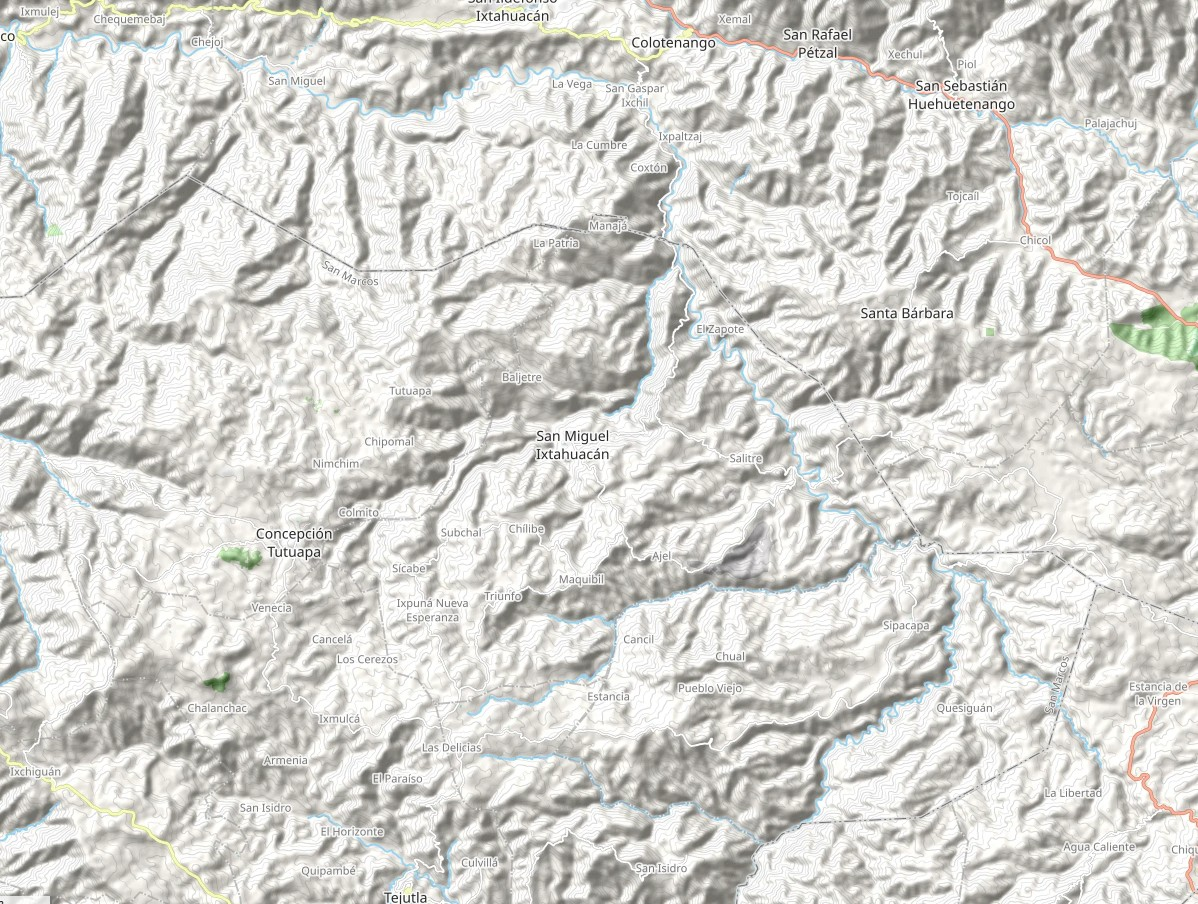
\includegraphics[width=0.85\textwidth]{imagenes/mapas/mapa_ubicacion_marlin.png}
%  \caption{Ubicación de la Mina Marlin, departamento de San Marcos, Guatemala}
%  \label{fig:mapa-ubicacion}
%  \par\vspace{2pt}
%  \raggedright\footnotesize Nota. Mapa base de OpenStreetMap,
%  \textcopyright{} OpenStreetMap contributors, licencia ODbL
%  \parencite{osmsfmapa}. Coordenadas del yacimiento:
%  15\textdegree14\textquotesingle05\textquotedbl{} N,
%  91\textdegree41\textquotesingle22\textquotedbl{} O.
%\end{figure}

% ---------------------------------------------------------------------
\subsection{Entorno social y económico}

La población de los municipios de San Miguel Ixtahuacán y Sipacapa asciende
conjuntamente a unos 70.000 habitantes y es mayoritariamente indígena: maya-mam
en San Miguel Ixtahuacán y maya-sipakapense en Sipacapa. La base económica
predominante es la agricultura de subsistencia
\parencite{oncommonground2010hria, ocmalsfmarlin}.

Este párrafo, breve en extensión, es el que sostiene toda la dimensión social del
informe y conviene explicitar por qué. Que el territorio afectado esté habitado
por pueblos indígenas no constituye un dato demográfico accesorio: es el hecho
jurídico que activa el Convenio 169 de la Organización Internacional del Trabajo
y el Performance Standard 7 de la Corporación Financiera Internacional, expuestos
ambos en la sección \ref{sec:marco} \parencite{oit1989convenio169}. Sin esa
condición, la ausencia de consulta previa sería una deficiencia de
relacionamiento comunitario; con ella, se convierte en el incumplimiento de una
obligación internacional exigible, que es exactamente como se clasifica en la
sección \ref{sec:hallazgos}.

A ello se añade un segundo factor, de naturaleza económica. Una población de
agricultura de subsistencia mantiene con el territorio una relación de dependencia
material directa: la tierra y el agua no son un entorno, son el medio de vida. La
consecuencia es que el umbral a partir del cual un impacto ambiental se percibe
como una amenaza existencial es mucho más bajo que en un entorno urbano o
industrializado. Esta asimetría en la percepción del riesgo, más que la magnitud
absoluta de los impactos medidos, explica buena parte de la persistencia del
conflicto y del desencuentro entre los monitoreos oficiales y la experiencia
comunitaria que se discute en la sección \ref{sec:critico}.

% ---------------------------------------------------------------------
\subsection{Marco geológico y mineralización}

La Mina Marlin explotó oro (Au) como producto principal y plata (Ag) como
coproducto de valor económico relevante. El yacimiento corresponde a un depósito
\textbf{epitermal de baja sulfuración de Au-Ag}, controlado estructuralmente por
la falla Virginia. La roca huésped está constituida por una unidad volcánica
máfica de edad terciaria y por tobas andesíticas pertenecientes al denominado
Complejo Marlin \parencite{sec2011ni43101}.

La mineralización se presenta en forma de vetas y de \textit{stockworks} de cuarzo
bandeado, calcita y adularia. La asociación mineralógica documentada incluye
pirita, acantita, pirargirita-proustita, y oro nativo y electrum. Esta composición
tiene una implicación ambiental que conviene señalar desde ahora: la presencia
significativa de pirita en la roca huésped y en el desmonte es la condición
geoquímica que genera el potencial de \textbf{drenaje ácido de roca}. Al quedar
expuesta la pirita a la acción del oxígeno y el agua, su oxidación produce
acidez, que a su vez moviliza metales pesados hacia las aguas superficiales y
subterráneas. El riesgo de drenaje ácido identificado por la auditoría no es, por
tanto, una contingencia operativa: es una consecuencia previsible de la geología
del yacimiento, y como tal debía haber sido anticipada desde el estudio de
impacto ambiental \parencite{moran2004review}.

Las estructuras mineralizadas se agrupan en varias vetas y zonas. La veta Virginia
concentró la producción subterránea histórica; junto a ella se reconocen las vetas
Rosa y Tello-Tomates. En el ámbito del tajo abierto se explotaron la zona Marlin
o \textit{Main Zone}, West Vero y La Hamaca, además del tajo satélite Cochis
\parencite{sec2011ni43101}.

La Tabla \ref{tab:reservas} resume las reservas y los recursos declarados en el
informe técnico NI 43-101. Debe leerse con una precaución metodológica: las
reservas no son una propiedad permanente del yacimiento, sino una estimación
referida a una fecha y a unos supuestos económicos determinados. Los valores que
se consignan tienen fecha efectiva de 31 de diciembre de 2010, es decir,
corresponden a la mitad de la vida útil de la operación y no a su totalidad.

% --- TABLA: Reservas y recursos --------------------------------------
\begin{table}[H]
  \centering
  \caption{Reservas y recursos declarados de la Mina Marlin (fecha efectiva: 31 de diciembre de 2010)}
  \label{tab:reservas}
  % \small y un \tabcolsep reducido: con seis columnas y cifras de ocho
  % dígitos, a tamaño normal la tabla se sale del margen.
  \begin{small}
  \setlength{\tabcolsep}{5pt}
  \begin{tabular}{@{}l r r r r r@{}}
    \toprule
    \textbf{Categoría} & \textbf{Tonelaje} & \textbf{Ley Au} & \textbf{Ley Ag}
      & \textbf{Au contenido} & \textbf{Ag contenida} \\
     & \textbf{(kt)} & \textbf{(\gt)} & \textbf{(\gt)}
      & \textbf{(\ozAu)} & \textbf{(\ozAg)} \\
    \midrule
    Reservas probadas y probables & 9.211 & 5,17 & 203,6 & 1.529.600 & 60.296.200 \\
    Recursos medidos e indicados\textsuperscript{a} & 922 & 1,78 & 78,8 & --- & --- \\
    \bottomrule
  \end{tabular}
  \end{small}
  \par\vspace{3pt}
  \raggedright\footnotesize
  Nota. \textsuperscript{a}Exclusivos de reservas. El informe técnico no reporta
  el contenido de metal de esta categoría; los guiones indican dato no
  disponible en la fuente, no ausencia de contenido metálico. Tomado de
  \textcite{sec2011ni43101}.
\end{table}
% NOTA PARA QUIEN EDITE: si quieres rellenar las dos celdas con «---», puedes
% calcularlas (tonelaje x ley / 31,1035 g por onza troy), pero DEBES indicar en
% la nota que son valores calculados y no tomados del informe técnico.

% ---------------------------------------------------------------------
\subsection{Método de explotación}

La Mina Marlin operó mediante un \textbf{método mixto}, combinando explotación a
tajo abierto y explotación subterránea. El tajo se desarrolló mediante bancos y
terrazas concéntricas, conforme a la configuración habitual en yacimientos de
este tipo. La explotación subterránea se realizó mediante una rampa en espiral de
4,6 m de ancho por 4,9 m de alto; hacia el final de la vida útil de la operación
se habían desarrollado aproximadamente 147 km de labores subterráneas
\parencite{sec2011ni43101}.

La coexistencia de ambos métodos generó dos perfiles de impacto claramente
diferenciados, y conviene distinguirlos porque las quejas comunitarias
documentadas en la auditoría se dirigen a uno y otro por separado.

El tajo abierto produce impactos de superficie: remoción de cobertura vegetal y
suelo, alteración del relieve, generación de grandes volúmenes de desmonte —con
el consiguiente potencial de drenaje ácido ya señalado—, emisión de material
particulado y vibraciones por voladura. Son impactos visibles, medibles y
relativamente fáciles de atribuir.

La explotación subterránea, en cambio, produce impactos menos evidentes pero de
atribución más disputada: subsidencia, alteración de los niveles freáticos y
vibraciones transmitidas por el macizo rocoso. El agrietamiento de viviendas en
las comunidades del entorno constituyó uno de los motivos de queja recurrentes de
la población, y es un caso ilustrativo de la dificultad probatoria que atraviesa
todo el expediente: establecer si una grieta obedece a la actividad minera, a la
sismicidad regional o a la calidad constructiva de la vivienda exige una línea
base y un monitoreo estructural previos que, de no existir, hacen la controversia
técnicamente irresoluble \parencite{oncommonground2010hria}. Este punto anticipa
uno de los ejes del análisis crítico de la sección \ref{sec:critico}: la ausencia
de línea base robusta no es un detalle técnico, sino la condición que perpetúa el
desacuerdo.

% ---------------------------------------------------------------------
\subsection{Procesamiento metalúrgico}

El circuito de beneficio empleado en Marlin corresponde al esquema convencional de
recuperación de oro y plata por cianuración, con recuperación final por
precipitación con zinc. La secuencia documentada es la siguiente
\parencite{sec2011ni43101}:

\begin{enumerate}
  \item \textbf{Trituración.} Reducción granulométrica primaria del mineral
        procedente del tajo y de la mina subterránea.
  \item \textbf{Molienda.} Molino SAG seguido de molino de bolas, hasta alcanzar
        una granulometría de 85 \% pasante la malla 200.
  \item \textbf{Lixiviación por agitación con cianuro}, en configuración de tipo
        CIL (\textit{carbon in leach}), en la que la disolución del oro y la plata
        y su adsorción sobre carbón activado ocurren simultáneamente.
  \item \textbf{Decantación en contracorriente}, para la separación y el lavado
        de la solución rica respecto de los sólidos.
  \item \textbf{Precipitación Merrill-Crowe con zinc}, que recupera los metales
        preciosos de la solución mediante cementación.
  \item \textbf{Fundición}, con obtención de barras doré de oro y plata como
        producto final comercializable.
  \item \textbf{Destrucción de cianuro} mediante el proceso INCO, aplicado a la
        pulpa antes de su depósito en la instalación de relaves.
\end{enumerate}

Dos aspectos de este circuito merecen comentario desde la perspectiva de la
auditoría. El primero es que el uso de cianuro constituye el aspecto ambiental
más significativo de toda la operación, en el sentido técnico que la
ISO 14001:2015 da a ese término y que se definió en la sección \ref{sec:marco}.
El segundo es que la operación incorporó un circuito específico de destrucción de
cianuro previo al depósito de relaves, y que fue la primera mina de Centroamérica
certificada bajo el \textit{International Cyanide Management Code}. Este dato es
relevante y debe consignarse con exactitud: acredita la adopción de un estándar
internacional voluntario en materia de manejo de cianuro, pero no equivale a una
certificación del desempeño ambiental global de la operación ni cubre los
riesgos de drenaje ácido, que tienen un origen geoquímico distinto y quedan fuera
del alcance de ese código. Confundir ambas cosas —una certificación específica
con una garantía general— es precisamente el tipo de inferencia que una auditoría
debe evitar.

% --- FIGURA 2: Diagrama de flujo del proceso -------------------------
% PENDIENTE DE INSERTAR. Puedes dibujarlo en TikZ o hacerlo en draw.io /
% PowerPoint y exportarlo a PDF (NO a JPG). Guárdalo en imagenes/diagramas/.
% Sigue la secuencia de los siete pasos enumerados arriba.
%\begin{figure}[H]
%  \centering
%  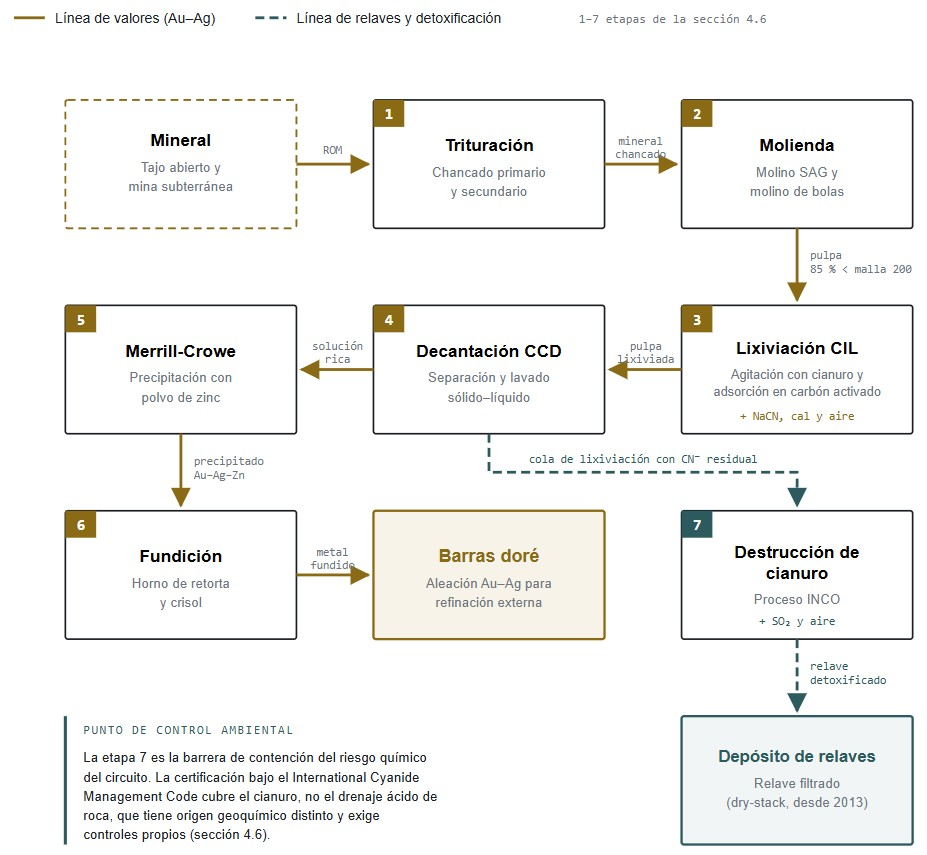
\includegraphics[width=0.9\textwidth]{imagenes/diagramas/flujo_proceso.pdf}
%  \caption{Diagrama de flujo del proceso metalúrgico de la Mina Marlin}
%  \label{fig:flujo-proceso}
%  \par\vspace{2pt}
%  \raggedright\footnotesize Nota. Elaboración propia a partir de
%  \textcite{sec2011ni43101}.
%\end{figure}

% ---------------------------------------------------------------------
\subsection{Capacidad de tratamiento: precisión sobre las cifras}

La capacidad de tratamiento de la planta es uno de los datos que con mayor
frecuencia aparece distorsionado en las fuentes secundarias sobre este caso, y su
tratamiento riguroso constituye en sí mismo un ejercicio de auditoría. No existe
una cifra única correcta: existen varias métricas distintas, cada una válida en
su propio marco, que solo pueden compararse si se declara a qué se refiere cada
una. La Tabla \ref{tab:capacidad} las presenta de forma explícita.

% --- TABLA: Capacidad de tratamiento ---------------------------------
\begin{table}[H]
  \centering
  \caption{Capacidad de tratamiento de la planta de la Mina Marlin según la métrica declarada}
  \label{tab:capacidad}
  \begin{tabularx}{\textwidth}{@{}L{4.3cm} L{3.3cm} Y@{}}
    \toprule
    \textbf{Métrica} & \textbf{Valor} & \textbf{Observación} \\
    \midrule
    Diseño nominal del molino & $\approx$1,82 Mt/año & Capacidad de diseño original. \\
    \addlinespace
    Capacidad optimizada & $\approx$2,05 Mt/año \newline ($\approx$5.000--5.600 \tdia) &
      Tras las mejoras introducidas en el circuito. \\
    \addlinespace
    Procesamiento real (2010) & $\approx$1,4 Mt/año \newline ($\approx$3.800 \tdia) &
      Tratamiento efectivo, inferior a la capacidad instalada. \\
    \addlinespace
    Rango operativo declarado en la venta de la planta & 4.000--7.000 \tdia \newline
      (promedio $\approx$6.000 \tdia) & Cifra del anuncio de venta del activo;
      procede de una fuente comercial, no técnica. \\
    \midrule
    \multicolumn{3}{@{}l}{\textit{Dato que NO corresponde a capacidad de planta:}} \\
    Material total minado & $\approx$24.282 \tdia &
      Incluye mineral \textbf{y} desmonte. No es capacidad de tratamiento. \\
    \bottomrule
  \end{tabularx}
  \par\vspace{3pt}
  \raggedright\footnotesize
  Nota. Elaboración propia a partir de \textcite{sec2011ni43101} y
  \textcite{miningcomsfventa}.
\end{table}

La distinción de la última fila es la más importante y la que con más frecuencia
se pasa por alto. La cifra aproximada de 24.282 \tdia\ que figura en el informe
técnico corresponde al \textbf{material total minado}, esto es, la suma del
mineral enviado a planta y del desmonte movido para acceder a él. Presentarla
como capacidad de tratamiento supone multiplicar por un factor de entre cuatro y
seis la capacidad real de la planta. Un informe de auditoría que incurriera en
esa confusión perdería credibilidad técnica en su conjunto, y por eso se deja
constancia expresa del punto.

Debe señalarse asimismo que la cuarta fila procede de un anuncio comercial de
venta del activo, no de un documento técnico sometido a estándar de reporte. Se
incluye por transparencia y porque es la fuente que sostiene las cifras más altas
que circulan sobre la operación, pero su jerarquía probatoria es inferior a la
del informe NI 43-101 y así debe ponderarse.

% ---------------------------------------------------------------------
\subsection{Producción, empleo y ciclo de vida de la operación}

A lo largo de sus doce años de operación, entre 2005 y 2017, la Mina Marlin
produjo \textbf{2,3 millones de onzas de oro y 63 millones de onzas de plata},
cifra confirmada por la propia empresa \parencite{goldcorp2017legacy}. Ello
equivale a un promedio anual del orden de 250.000 \ozAu\ y 3,5 millones de
\ozAg. La operación fue la mayor mina y la principal exportadora de oro de
Guatemala y de Centroamérica.

En cuanto al empleo, la operación alcanzó un máximo aproximado de 3.000
trabajadores en su fase de mayor actividad. En operación plena se estimaban
alrededor de 2.000 empleos directos y unos 8.000 indirectos. Al momento del
cierre, la plantilla se había reducido a unos 1.200 trabajadores
\parencite{oncommonground2010hria, prensalibre2017cierre}.

Estas magnitudes conviene interpretarlas, no solo enunciarlas. El eje de
inversión económica y social de la auditoría reconoció que la operación generó
aportes efectivos en empleo e ingresos, y las cifras anteriores lo confirman. Pero
el mismo eje concluyó que la mitigación de los impactos negativos resultó
insuficiente. Ambas afirmaciones son compatibles y su coexistencia es
precisamente el núcleo del problema: la magnitud del beneficio agregado no
compensa automáticamente la distribución desigual de los perjuicios, sobre todo
cuando beneficios y perjuicios recaen sobre poblaciones distintas y en horizontes
temporales distintos. El empleo dura lo que dura la mina —doce años— mientras que
el pasivo ambiental permanece indefinidamente. Esta asimetría temporal es la que
convierte la planificación del cierre y del post-cierre, tratada en la sección
\ref{sec:plan}, en la cuestión decisiva del caso.

El cierre de producción se produjo el 31 de mayo de 2017 e incluyó un plan de
recuperación ambiental con destrucción de cianuro y relleno del tajo
\parencite{goldcorp2023marlin}. Que la operación haya completado su ciclo
íntegro —construcción, operación, conflicto, auditoría, plan de acción, cierre y
post-cierre— es lo que permite a este informe evaluar la mejora continua sobre un
caso cerrado y no sobre una operación todavía en curso.

% ---------------------------------------------------------------------
\subsection{Infraestructura crítica y gestión de relaves}

La instalación de mayor criticidad ambiental de la operación fue el depósito de
relaves (\textit{tailings storage facility}), construido entre 2004 y 2010 en el
valle situado al norte de la planta de proceso. Con posterioridad, la operación
inició la transición hacia un esquema de relaves filtrados o apilamiento en seco
(\textit{dry-stack}), mediante una planta de filtrado de marca Metso instalada en
2013 y operativa hasta el cierre en 2017 \parencite{sec2011ni43101}.

Esta transición merece una valoración positiva explícita, porque constituye uno de
los pocos elementos del expediente en que la operación se adelantó a la evolución
del estándar sectorial. El apilamiento en seco reduce sustancialmente el riesgo
de rotura catastrófica al eliminar el embalse de agua que caracteriza a los
depósitos convencionales, que es precisamente el mecanismo que produjo los
colapsos de Mount Polley, Samarco y Brumadinho. Que Marlin iniciara esa
transición en 2013 —seis años antes de Brumadinho y siete antes de la publicación
del Global Industry Standard on Tailings Management— es un dato que el análisis
debe reconocer con la misma objetividad con que consigna las deficiencias
\parencite{icmm2020gistm}.

La operación contó además con una planta de tratamiento de agua, puesta en
servicio en 2008, y con un aliviadero de emergencia dimensionado para la Crecida
Máxima Probable, cuya construcción supuso una inversión aproximada de US\$ 14
millones y más de 8.000 m\textsuperscript{3} de concreto. En materia de
verificación, el depósito fue objeto de revisiones quinquenales de seguridad de
presa conforme a los protocolos de la Canadian Dam Association, realizadas por
Tierra Group International \parencite{sec2011ni43101}.

\subsubsection{Limitación de información declarada}

Es preciso dejar constancia expresa de una limitación en la información
disponible. No fue posible verificar, en fuente primaria específica de la Mina
Marlin, tres parámetros básicos del depósito de relaves: el \textbf{tipo
constructivo de la presa} —aguas arriba, aguas abajo o de línea central—, su
\textbf{altura} y su \textbf{volumen almacenado}. Estos datos requerirían el
acceso al estudio de impacto ambiental detallado o al informe de diseño de
ingeniería de la instalación.

La omisión es deliberada y conviene justificarla, porque un lector podría
interpretarla como una laguna de la investigación. En primer lugar, el método
constructivo de una presa de relaves es el parámetro que más determina su perfil
de riesgo: fue el método aguas arriba el que falló por licuefacción estática en
Brumadinho \parencite{robertson2019feijao}. Atribuir a Marlin un método
constructivo no verificado sería, por tanto, comprometer el hallazgo más sensible
del análisis sobre la base de una conjetura. En segundo lugar, sobre este caso
circulan en fuentes secundarias cifras que corresponden en realidad a otras
operaciones mineras, de modo que el riesgo de contaminación de datos es real y
documentado. Declarar la limitación es metodológicamente preferible a rellenarla
con una cifra plausible: en auditoría, la ausencia de evidencia se registra como
tal y no se sustituye por inferencia.

Finalmente, cabe señalar que durante el período de operación no existía todavía un
estándar internacional específico y auditable para la gestión de relaves. El
GISTM se publicó en 2020, tres años después del cierre. La gestión del depósito se
verificaba, en consecuencia, contra protocolos privados y guías nacionales de
terceros países, como los de la Canadian Dam Association ya mencionados. Esta
circunstancia debe tenerse presente al valorar los hallazgos ambientales de la
sección \ref{sec:hallazgos}: la vara de medir disponible en su momento era
sustancialmente menos exigente que la actual, lo que no exime de responsabilidad
pero sí obliga a evaluar la conducta contra los criterios vigentes entonces y no
contra los de hoy.
     % Integrante 2
% =====================================================================
%  5. DESCRIPCIÓN DE LA AUDITORÍA  <- NÚCLEO DEL TRABAJO
%  Responsable: INTEGRANTE 3
%  ESTADO: REDACTADO (1 de agosto de 2026) — ~2.300 palabras + 2 tablas
%  Fuente principal: Sección C de docs/bitacora_decisiones.md
%  Documento ancla: HRIA de On Common Ground (PDF espejado en q4cdn.com)
%
%  Contiene la Tabla del equipo auditor y la Tabla de criterios de
%  auditoría. Falta insertar la Figura 3 (línea de tiempo): el entorno
%  está listo y comentado al final del archivo.
%
%  ENFOQUE MANTENIDO: esta sección DESCRIBE la auditoría. La evaluación
%  crítica va en la sección 7. Donde aparece un dato incómodo —el
%  financiamiento por la empresa auditada, la no ejecución de la revisión
%  por pares, la ausencia de Sipacapa— se consigna como HECHO y se remite
%  a la sección 7, sin juzgarlo aquí. Ese orden es lo que distingue un
%  informe de auditoría de un alegato.
% =====================================================================

\section{Descripción de la auditoría}
\label{sec:auditoria}

Esta sección reconstruye el proceso de auditoría analizado: quién lo promovió,
quién lo ejecutó, con qué mandato, contra qué criterios y mediante qué método. El
documento examinado es la \hria, elaborada por \auditora\ y publicada en mayo de
2010 \parencite{oncommonground2010hria}.

La exposición se atiene deliberadamente a un registro descriptivo. Varios de los
hechos que se consignan a continuación —que la evaluación fue financiada por la
empresa auditada, que la revisión por pares prevista no llegó a ejecutarse, o que
la participación del municipio de Sipacapa resultó insuficiente— admiten una
lectura crítica que se desarrolla en la sección \ref{sec:critico}. Separar ambos
planos no es una formalidad: una auditoría se evalúa comparando lo que se hizo
con lo que debió hacerse, y para ello es imprescindible establecer primero, sin
valoración, qué fue exactamente lo que se hizo.

% ---------------------------------------------------------------------
\subsection{Antecedentes y origen del encargo}

El rasgo más singular de este proceso es su origen. La evaluación no fue iniciativa
de la empresa ni orden de una autoridad estatal, sino resultado de la presión
ejercida por un grupo de \textbf{accionistas socialmente responsables} sobre la
matriz corporativa. Los promotores fueron Ethical Funds, el First Swedish
National Pension Fund, el Fourth Swedish National Pension Fund, el Public Service
Alliance of Canada Staff Pension Fund y SHARE
\parencite{oncommonground2010hria}.

Esa vía de activación merece atención analítica. En el esquema clásico de control
ambiental expuesto en la sección \ref{sec:marco}, la verificación de la conducta
empresarial procede del Estado, mediante fiscalización, o del mercado de la
certificación, mediante auditorías de tercera parte. Aquí operó un tercer
mecanismo: el capital accionario. Fueron inversionistas institucionales quienes,
en ejercicio de sus políticas de inversión responsable, condicionaron su relación
con la empresa a que esta se sometiera a una evaluación independiente de derechos
humanos. Se trata de un mecanismo de gobernanza privada que no sustituye a la
fiscalización estatal —carece de potestad sancionadora— pero que en este caso
consiguió lo que aquella no había logrado: que la operación fuese examinada por un
tercero externo y que el resultado se hiciera público.

El contexto que hizo posible esa presión estaba ya formado. En 2005 la
organización no gubernamental Madre Selva había presentado una queja ante la
Compliance Advisor Ombudsman de la Corporación Financiera Internacional respecto
del préstamo otorgado al proyecto, procedimiento que concluyó en mayo de 2006
\parencite{cao2006marlin}. El conflicto social en San Miguel Ixtahuacán y
Sipacapa estaba plenamente instalado, la consulta comunitaria de Sipacapa se había
celebrado en 2005, y la revisión independiente del estudio de impacto ambiental
elaborada por \textcite{moran2004review} circulaba desde 2004. La evaluación de
derechos humanos no surgió, por tanto, en un escenario neutro, sino como respuesta
a un cuestionamiento previo y sostenido.

El proceso se formalizó mediante un \textbf{Memorando de Entendimiento} suscrito en
marzo de 2008. Para su gobierno se constituyó un \textbf{Comité Directivo}
(\textit{Steering Committee}) independiente, integrado por Bob Walker, Manfredo
Marroquín y Dave Deisley, con la participación de Bill Brassington. Fue ese comité
—y no la dirección de la empresa— el que en octubre de 2008 seleccionó a la firma
auditora \parencite{oncommonground2010hria}. La interposición de una instancia
independiente entre quien financia y quien audita es un elemento de diseño
institucional deliberado, cuyo alcance y cuyas limitaciones se discuten en la
sección \ref{sec:critico}.

% ---------------------------------------------------------------------
\subsection{Organismo auditor, mandato y financiamiento}

La evaluación fue ejecutada por \auditora, consultora independiente con sede en
Vancouver, Canadá, especializada en evaluación social y relacionamiento
comunitario en el sector minero \parencite{oncommonground2010hria}.

El encargo procedió del Comité Directivo de la evaluación, actuando «en nombre de
Goldcorp». El \textbf{financiamiento corrió íntegramente a cargo de Goldcorp}, es
decir, de la matriz de la empresa auditada. Este dato se consigna aquí como hecho
verificado y sin valoración; su análisis corresponde a la sección
\ref{sec:critico}. Conviene únicamente advertir que la circunstancia no es
excepcional en el ámbito de las evaluaciones de impacto en derechos humanos:
prácticamente todas se financian de ese modo, sencillamente porque no existe un
mecanismo alternativo de financiación consolidado. Lo que distingue a un proceso
de otro no es la ausencia de esa dependencia, sino las salvaguardas que se
articulan frente a ella.

En este caso, tales salvaguardas fueron tres, todas ellas fijadas por escrito en el
Memorando de Entendimiento. La primera es el conjunto de principios rectores del
proceso: \textbf{transparencia, independencia e inclusividad}. La segunda es la
interposición del Comité Directivo como órgano de selección y supervisión. La
tercera es el compromiso de publicación íntegra del informe, incluidos los
hallazgos desfavorables a la empresa; compromiso que efectivamente se cumplió, y
que explica que este trabajo pueda apoyarse en un documento público de más de
doscientas páginas.

A estos principios el propio equipo auditor añadió, en diciembre de 2008, dos
principios éticos adicionales de su propia iniciativa: el \textbf{consentimiento
informado} de las personas entrevistadas y la \textbf{confidencialidad} de sus
declaraciones \parencite{oncommonground2010hria}. La incorporación no es un
detalle menor. En una auditoría desarrollada en un territorio en conflicto, donde
quienes testimonian pueden sufrir represalias, la confidencialidad no es una
cortesía procedimental sino una condición material para que exista testimonio. Se
corresponde, además, con el principio de confidencialidad que la ISO 19011:2018
exige a todo auditor \parencite{iso2018iso19011}.

% ---------------------------------------------------------------------
\subsection{Composición y competencia del equipo auditor}

La ISO 19011:2018 exige que la competencia del equipo auditor se determine y
evalúe en función de los conocimientos y habilidades necesarios para alcanzar los
objetivos de la auditoría \parencite{iso2018iso19011}. Procede, en consecuencia,
examinar si el perfil del equipo cubría las dos dimensiones —social y ambiental—
comprendidas en su alcance. La Tabla \ref{tab:equipo-auditor} resume su
composición.

% --- TABLA: Composición del equipo auditor ---------------------------
\begin{table}[H]
  \centering
  \caption{Composición del equipo de la evaluación de derechos humanos de la Mina Marlin}
  \label{tab:equipo-auditor}
  \begin{small}
  \begin{tabularx}{\textwidth}{@{}L{3.6cm} L{3.4cm} Y@{}}
    \toprule
    \textbf{Integrante} & \textbf{Rol} & \textbf{Perfil y aporte} \\
    \midrule
    Susan Joyce & Líder del equipo &
      Socióloga con más de 25 años de experiencia en aspectos sociales de la
      minería y en derechos humanos. \\
    \addlinespace
    Myriam Cabrera & Equipo principal & Evaluación social y trabajo de campo. \\
    \addlinespace
    Giselle Huamani & Equipo principal &
      Experiencia regional en transformación de conflictos socioambientales. \\
    \addlinespace
    Lloyd Lipsett & Equipo principal &
      Marco jurídico de empresas y derechos humanos. \\
    \addlinespace
    Monica Leonardo Segura & Apoyo & Contexto jurídico guatemalteco. \\
    \addlinespace
    Sandro Macassi & Apoyo & Análisis de conflictos y comunicación. \\
    \addlinespace
    International Alert & Revisión por pares &
      \textbf{Prevista en el diseño, no ejecutada según lo planeado.} \\
    \bottomrule
  \end{tabularx}
  \end{small}
  \par\vspace{3pt}
  \raggedright\footnotesize
  Nota. Los perfiles de los integrantes distintos de la líder del equipo se
  describen de forma resumida; el informe original no detalla la trayectoria
  individual de cada uno. Elaboración propia a partir de
  \textcite{oncommonground2010hria}.
\end{table}

Del cuadro se desprenden dos observaciones de carácter descriptivo. La primera es
que el equipo reunía un perfil predominantemente \textbf{social y jurídico}:
sociología, derechos humanos, análisis de conflictos y derecho. No incorporaba
especialistas en hidrogeología, geoquímica ni ingeniería de relaves. Esta
composición es coherente con el objeto declarado de la evaluación —una evaluación
de impactos en derechos humanos, no una auditoría técnico-ambiental— y el equipo
resolvió la brecha por la vía de encargar una revisión ambiental independiente,
según se detalla en la subsección de metodología.

La segunda observación se refiere a la revisión por pares. El diseño del proceso
contemplaba que International Alert, organización con sede en Londres
especializada en construcción de paz, ejerciera de revisor par del trabajo. Esa
revisión \textbf{no llegó a ejecutarse según lo previsto}. Se consigna aquí como
hecho, por su relevancia para la valoración de la calidad del proceso, que se
aborda en la sección \ref{sec:critico}.

% ---------------------------------------------------------------------
\subsection{Alcance de la auditoría}

El alcance temporal de la evaluación se extendió desde el momento en que Glamis
Gold asumió la condición de operadora hasta la fecha de emisión del informe, en
mayo de 2010, e incorporó además una mirada prospectiva sobre el cierre y el
post-cierre de la operación. El alcance espacial quedó circunscrito al área de la
licencia de explotación \parencite{oncommonground2010hria}.

Junto al alcance, el informe declaró expresamente una \textbf{limitación}: la
participación del municipio de Sipacapa y de los sectores opositores a la mina
resultó insuficiente, por lo que los propios auditores calificaron sus hallazgos
sobre impactos como parciales.

El registro de esta limitación exige una precisión conceptual que enlaza
directamente con la sección \ref{sec:marco}. En la lógica de la ISO 19011:2018, el
alcance y sus exclusiones no son un preámbulo administrativo: condicionan la
validez de las conclusiones. Si la auditoría se sustenta en un enfoque basado en
la evidencia, y la evidencia se obtiene mediante muestreo, entonces la
representatividad de la muestra determina hasta dónde alcanzan las conclusiones
\parencite{iso2018iso19011}. Una evaluación de impactos sociales que no logra
incorporar el testimonio de la población más crítica no obtiene una muestra
incompleta en sentido meramente cuantitativo: obtiene una muestra sesgada en la
dirección precisa que importa. Cuál sea el peso de ese sesgo se discute en la
sección \ref{sec:critico}; aquí basta con dejar constancia de que los auditores lo
declararon ellos mismos, lo que constituye, en sí, una práctica correcta.

% ---------------------------------------------------------------------
\subsection{Criterios de auditoría aplicados}

Los criterios de auditoría son la vara de medir: el conjunto de requisitos frente
a los cuales se compara la conducta observada. Su elección determina qué puede
llegar a constituir un hallazgo y qué queda, por definición, fuera del examen. La
Tabla \ref{tab:criterios} sistematiza los criterios aplicados en esta evaluación,
distinguiendo su naturaleza jurídica.

% --- TABLA: Criterios de auditoría -----------------------------------
\begin{table}[H]
  \centering
  \caption{Criterios de auditoría aplicados en la evaluación de la Mina Marlin}
  \label{tab:criterios}
  \begin{small}
  \begin{tabularx}{\textwidth}{@{}L{5.2cm} L{3.2cm} Y@{}}
    \toprule
    \textbf{Criterio} & \textbf{Naturaleza} & \textbf{Ámbito que gobierna} \\
    \midrule
    Declaración Universal de Derechos Humanos & Marco internacional &
      Referencia general de derechos. \\
    \addlinespace
    Pacto Internacional de Derechos Civiles y Políticos & Tratado vinculante &
      Seguridad personal, libertad de asociación. \\
    \addlinespace
    Pacto Internacional de Derechos Económicos, Sociales y Culturales &
      Tratado vinculante & Agua, salud, trabajo, medios de vida. \\
    \addlinespace
    Convenio 169 de la {OIT} & Tratado vinculante para el Estado &
      Consulta previa, libre e informada; tierras. \\
    \addlinespace
    Marco «Proteger, Respetar, Remediar» (Ruggie) & Marco de referencia &
      Estructura general del análisis. \\
    \addlinespace
    Herramienta {HRCA} del {DIHR} & Herramienta metodológica &
      Instrumento de verificación, adaptado al caso. \\
    \addlinespace
    {IFC} Performance Standards & Obligación contractual &
      Exigibles por el préstamo de la {IFC}. \\
    \addlinespace
    {ICMM} Mining Principles & Estándar voluntario sectorial &
      Desempeño corporativo. \\
    \addlinespace
    Principios Voluntarios en Seguridad y Derechos Humanos & Estándar voluntario &
      Seguridad privada y pública. \\
    \bottomrule
  \end{tabularx}
  \end{small}
  \par\vspace{3pt}
  \raggedright\footnotesize
  Nota. Elaboración propia a partir de \textcite{oncommonground2010hria}.
\end{table}

La columna central de la tabla revela un rasgo estructural del caso. Los criterios
aplicados pertenecen a tres categorías de muy distinta exigibilidad. Los tratados
internacionales de derechos humanos y el Convenio 169 vinculan al \textbf{Estado
guatemalteco}, no directamente a la empresa. Los IFC Performance Standards
vinculan a la empresa, pero por vía \textbf{contractual}, como condición del
préstamo \parencite{ifcsfmarlin}. Los estándares del ICMM y los Principios
Voluntarios son de adhesión \textbf{voluntaria}. Ninguno de ellos es, en sentido
estricto, una norma sancionable directamente frente al operador por un órgano
administrativo, como sí lo sería el marco peruano expuesto en la sección
\ref{sec:marco}. Esta configuración explica por qué el resultado del proceso
fueron recomendaciones y no medidas correctivas exigibles.

Corresponde señalar, además, una diferencia de fondo respecto de la práctica
auditora convencional. Los criterios empleados son criterios de
\textbf{desempeño} en derechos humanos, no requisitos de un \textbf{sistema de
gestión}. La evaluación no fue una auditoría de certificación conforme a la
ISO 14001:2015 ni pretendió serlo. La consecuencia práctica es que sus resultados
no se formularon como no conformidades en el sentido técnico de la norma, lo que
obliga a este informe a construir una clasificación propia para el análisis de la
sección \ref{sec:hallazgos}. Explicitar esa diferencia evita atribuir a la
evaluación una naturaleza que no tuvo.

% ---------------------------------------------------------------------
\subsection{Metodología y cronograma}

La evaluación se desarrolló entre octubre de 2008 y mayo de 2010, esto es, a lo
largo de aproximadamente diecinueve meses, y se articuló en cinco líneas de
trabajo \parencite{oncommonground2010hria}:

\begin{enumerate}
  \item \textbf{Revisión de políticas, procedimientos y prácticas} de la empresa,
        contrastando el marco formal declarado con su aplicación efectiva.
  \item \textbf{Análisis de datos secundarios y consulta a fuentes expertas},
        incorporando información previamente producida por terceros.
  \item \textbf{Entrevistas individuales y grupales} con múltiples grupos de
        interés: trabajadores, autoridades, comunidades, organizaciones sociales y
        personal de la empresa.
  \item \textbf{Adaptación de la herramienta Human Rights Compliance Assessment}
        del Danish Institute for Human Rights, ajustada a las circunstancias del
        caso.
  \item \textbf{Revisión técnica ambiental independiente}, encargada por el propio
        equipo dentro del proceso de evaluación.
\end{enumerate}

La quinta línea merece un comentario específico, porque es la que convierte a este
proceso en el caso idóneo para el objeto de este informe. Un equipo de perfil
social y jurídico, consciente de la brecha de competencia técnica señalada
anteriormente, subcontrató la pericia ambiental en lugar de eludir la materia o de
pronunciarse sobre ella sin respaldo. Esa decisión metodológica es la que hace de
la evaluación un ejercicio efectivamente \textbf{socioambiental} y no únicamente
social, y es coherente con lo que la ISO 19011:2018 prevé cuando el equipo
auditor requiere conocimientos especializados de los que carece
\parencite{iso2018iso19011}.

\subsubsection{Contraste con las fases de la ISO 19011:2018}

Resulta ilustrativo mapear el proceso efectivamente seguido contra la secuencia de
fases que establece la norma de referencia, expuesta en la sección
\ref{sec:marco}. El ejercicio permite identificar dónde el proceso fue sólido y
dónde quedó débil.

El \textbf{inicio de la auditoría} está documentado con inusual precisión: existe
un memorando de entendimiento escrito, un órgano de gobierno constituido, un
procedimiento de selección del auditor y un conjunto de principios pactados. Es,
probablemente, la fase mejor resuelta del proceso.

La \textbf{revisión de la documentación} y la \textbf{preparación} se corresponden
con las líneas de trabajo primera y segunda, y la adaptación de la herramienta
HRCA equivale a la elaboración de los documentos de trabajo que la norma prevé.

Las \textbf{actividades de recolección de evidencia} se ejecutaron mediante
entrevistas, análisis documental y la revisión técnica encargada, cubriendo las
tres modalidades que la norma contempla. Es en esta fase, sin embargo, donde se
localiza la debilidad declarada: el muestreo de personas entrevistadas no alcanzó
la cobertura prevista respecto de Sipacapa y de los sectores opositores.

El \textbf{informe} se elaboró y se publicó íntegramente, en versión bilingüe, lo
que satisface con holgura el requisito de comunicación de resultados.

El \textbf{seguimiento} constituye el punto más problemático del contraste. La
norma concibe la auditoría como un ciclo que se cierra verificando la
implementación efectiva de las acciones correctivas. Aquí la empresa se comprometió
a emitir una respuesta pública y un plan de acción, con actualizaciones
publicadas en 2010, 2011 y 2017 \parencite{oncommonground2010hria,
goldcorp2023marlin}, pero la verificación de ese cumplimiento quedó en manos de la
propia empresa, sin que el equipo auditor original conservara mandato para
comprobarlo. La cuestión de si las no conformidades llegaron efectivamente a
cerrarse se retoma en las secciones \ref{sec:hallazgos} y \ref{sec:critico}.

% --- FIGURA 3: Línea de tiempo (dibujada en TikZ) --------------------
\begin{figure}[H]
  \centering
  \begin{tikzpicture}[
      hito/.style={circle,fill=azuloscuro,inner sep=1.4pt},
      arr/.style={-{Stealth[length=2.5mm]},very thick,azuloscuro},
      anio/.style={font=\scriptsize\bfseries,anchor=north,inner sep=1.5pt},
      arriba/.style={font=\scriptsize,align=center,anchor=south,inner sep=2pt},
      abajo/.style={font=\scriptsize,align=center,anchor=north,inner sep=2pt}
    ]
    % Eje
    \draw[arr] (-0.4,0) -- (14.2,0);

    % Hitos y años, pegados al eje
    \foreach \x/\y in {0/2004, 1.3/2005, 2.6/2006, 4.3/2008, 5.5/2009,
                       6.7/2010, 8.3/2011, 13.4/2017} {
      \node[hito] at (\x,0) {};
      \node[anio] at (\x,-0.14) {\y};
    }

    % Etiquetas por encima del eje
    \node[arriba] at (0,0.14)   {Revisión\\independiente\\del EIA};
    \node[arriba] at (2.6,0.14) {Cierre del\\caso CAO};
    \node[arriba] at (5.5,0.14) {Trabajo\\de campo};
    \node[arriba] at (8.3,0.14) {La CIDH retira\\la solicitud\\de suspensión};

    % Etiquetas por debajo, dejando sitio a la fila de años
    \node[abajo] at (1.3,-0.62)  {Consulta de\\Sipacapa;\\queja ante\\la CAO};
    \node[abajo] at (4.3,-0.62)  {MOU (mar.)\\Selección de\\la auditora\\(oct.)};
    \node[abajo] at (6.7,-0.62)  {\textbf{Publicación}\\\textbf{de la HRIA}\\(mayo)\\Medidas CIDH\\OIT/CEACR};
    \node[abajo] at (13.4,-0.62) {Cierre de\\la mina\\(31 mayo)};

    % Duración del proceso de auditoría
    \draw[azuloscuro,thick,|-|] (4.3,1.55) -- (6.7,1.55)
      node[midway,above,font=\scriptsize] {Proceso de auditoría (19 meses)};
  \end{tikzpicture}
  \caption{Cronología del proceso de auditoría de la Mina Marlin (2004--2017)}
  \label{fig:metodologia}
  \par\vspace{2pt}
  \raggedright\footnotesize
  Nota. El eje no es estrictamente proporcional entre 2011 y 2017.
  Elaboración propia a partir de \textcite{oncommonground2010hria},
  \textcite{cao2006marlin} y \textcite{cidh2010medidas}.
\end{figure}
         % Integrante 3
% =====================================================================
%  6. ANÁLISIS DE HALLAZGOS  <- LA SECCIÓN QUE MÁS CALIFICA
%  Responsable: INTEGRANTE 4
%  ESTADO: REDACTADO (1 de agosto de 2026) — ~3.700 palabras + matriz completa
%  Fuentes: HRIA + CAO/IFC + estudio de salud PHR/Michigan + monitoreo COPAE
%
%  LA MATRIZ (Tabla 6) ESTÁ COMPLETA, con diez hallazgos sobre los siete
%  ejes de la auditoría. Va en página apaisada y usa longtable.
%
%  DECISIONES METODOLÓGICAS QUE CONVIENE NO DESHACER:
%
%  1) El eje ambiental se DESDOBLA en tres hallazgos distintos: la
%     insuficiencia del monitoreo y de la línea base (que sí es
%     demostrable), la afectación efectiva del agua (que NO lo es, porque
%     la evidencia está en conflicto) y la planificación del cierre.
%     Meterlos en una sola fila obligaría a clasificar como incumplimiento
%     algo que no está probado, o a rebajar algo que sí lo está.
%
%  2) La columna «Estado de cierre» dice «no verificable» en la mayoría de
%     las filas. NO es una laguna del trabajo: es el hallazgo de la
%     sección 6.7. La empresa publicó actualizaciones de su plan de acción
%     en 2010, 2011 y 2017, pero no consta verificación independiente del
%     cierre de cada recomendación.
%
%  3) Se usa el condicional al describir el hallazgo laboral («habría
%     desalentado») porque así lo formula la fuente. No lo conviertas en
%     afirmación categórica sin ir al informe original.
% =====================================================================

\section{Análisis de hallazgos}
\label{sec:hallazgos}

Esta sección sistematiza los resultados de la auditoría analizada y los convierte
en hallazgos clasificados. Se organiza en tres movimientos: primero se declara la
regla de clasificación empleada; después se presenta la matriz completa de
hallazgos sobre los siete ejes evaluados; y finalmente se desarrollan en prosa los
cuatro hallazgos de mayor gravedad, aquellos que explican por sí solos la
trayectoria del caso.

% ---------------------------------------------------------------------
\subsection{Criterio de clasificación de los hallazgos}

Antes de clasificar es obligado explicitar con qué regla se clasifica. Un auditor
que aplica categorías sin haberlas definido convierte su juicio en
inverificable, que es exactamente lo contrario de lo que persigue el principio de
enfoque basado en la evidencia.

Debe advertirse, en primer lugar, que la evaluación analizada \textbf{no clasificó
sus resultados como no conformidades}. No era una auditoría de sistema de gestión
sino una evaluación de impactos en derechos humanos, según se estableció en la
sección \ref{sec:auditoria}, y sus resultados se formularon como hallazgos y
recomendaciones por ejes temáticos. La clasificación que se presenta a
continuación es, por tanto, una \textbf{adaptación propia} construida sobre las
definiciones de la ISO 19011:2018 expuestas en la sección \ref{sec:marco}
\parencite{iso2018iso19011}. Reconocerlo no debilita el análisis: lo hace
auditable.

La regla aplicada es la siguiente:

\begin{itemize}
  \item \NCmayor: incumplimiento de un requisito que afecta derechos
        fundamentales, o que tiene carácter sistémico por comprometer la
        capacidad del conjunto del sistema de gestión para producir resultados
        conformes.
  \item \NCmenor: incumplimiento puntual, acotado y subsanable, que no
        compromete la integridad del sistema.
  \item \OBS: situación en la que no existe incumplimiento demostrado, pero se
        identifica un riesgo relevante o una oportunidad de mejora. Se emplea
        también cuando la evidencia disponible es contradictoria y no permite
        concluir.
\end{itemize}

La tercera categoría requiere una precisión, porque su uso en este caso es
deliberado y no evasivo. Cuando dos cuerpos de evidencia técnica apuntan en
direcciones opuestas y ninguno puede descartarse, el auditor no está autorizado a
elegir el que confirme su hipótesis. Registrar una observación es, en esa
situación, la única conclusión que la evidencia sostiene.

Finalmente, se entiende por \textbf{evidencia objetiva}, en un análisis de
naturaleza documental como el presente, cualquiera de estas tres fuentes: el
contenido del propio informe de auditoría, un dato de monitoreo ambiental o
sanitario procedente de un estudio identificable, o el pronunciamiento formal de
un órgano oficial nacional o internacional.

% ---------------------------------------------------------------------
\subsection{Matriz de hallazgos y no conformidades}

La Tabla \ref{tab:matriz-nc} presenta los diez hallazgos identificados sobre los
siete ejes evaluados. Su distribución es la siguiente: cinco no conformidades
mayores, cuatro menores y una observación.

Conviene señalar por qué el eje ambiental aparece desdoblado en tres filas. La
insuficiencia del monitoreo y de la línea base es un hecho documentado y
constituye por sí misma un incumplimiento. La afectación efectiva de la calidad
del agua, en cambio, es objeto de evidencia contradictoria y no puede afirmarse
como incumplimiento. Y la planificación del cierre presenta un estado distinto de
ambas. Agrupar las tres cuestiones en un único hallazgo obligaría a dar por
probado lo que no lo está, o a rebajar lo que sí lo está.

\begin{landscape}
\begin{footnotesize}
\setlength{\tabcolsep}{4pt}
\begin{longtable}{@{}L{1.7cm} L{4.2cm} L{4.6cm} L{2.9cm} L{1.6cm} L{4.4cm} L{3.2cm}@{}}
  \caption{Matriz de hallazgos y no conformidades de la auditoría socioambiental de la Mina Marlin}
  \label{tab:matriz-nc} \\
  \toprule
  \textbf{Eje} & \textbf{Hallazgo} & \textbf{Evidencia objetiva} &
  \textbf{Criterio incumplido} & \textbf{Clasif.} & \textbf{Recomendación} &
  \textbf{Estado de cierre} \\
  \midrule
  \endfirsthead
  \multicolumn{7}{@{}l}{\textit{Tabla \ref{tab:matriz-nc} (continuación)}} \\[2pt]
  \toprule
  \textbf{Eje} & \textbf{Hallazgo} & \textbf{Evidencia objetiva} &
  \textbf{Criterio incumplido} & \textbf{Clasif.} & \textbf{Recomendación} &
  \textbf{Estado de cierre} \\
  \midrule
  \endhead
  \bottomrule
  \multicolumn{7}{@{}p{23cm}}{\textit{Nota.} Elaboración propia a partir de
  \textcite{oncommonground2010hria}, \textcite{cao2006marlin},
  \textcite{cidh2010medidas}, \textcite{basu2010scitotenv} y
  \textcite{etech2010water}. La clasificación es una adaptación propia
  construida sobre \textcite{iso2018iso19011}; la evaluación original no
  clasificó sus resultados como no conformidades.} \\
  \endlastfoot

  % --- 1. CONSULTA ---
  Consulta &
  La operación fue autorizada sin un proceso de consulta previa, libre e informada
  adecuado a la población maya-mam y maya-sipakapense &
  Constatación expresa de la evaluación; pronunciamiento de la {CEACR} de la
  {OIT} (2010) instando a suspender actividades hasta cumplir la consulta &
  Convenio 169 {OIT}, art. 6; {IFC} {PS}7 &
  \NCmayor &
  Detener la adquisición de tierras, la exploración y toda expansión hasta
  consultar debidamente &
  \textbf{No cerrada.} La operación continuó hasta 2017 \\
  \addlinespace

  % --- 2. AMBIENTE (a) ---
  Ambiente &
  Sistema de monitoreo ambiental y línea base insuficientes para atribuir o
  descartar impactos &
  Revisión independiente del {EIA} \parencite{moran2004review}; recomendación de
  la propia evaluación de reforzar el monitoreo &
  {IFC} {PS}1 &
  \NCmayor &
  Reforzar el monitoreo, incluida la participación comunitaria a través de la
  {AMAC} &
  \textbf{Parcial.} Planta de tratamiento de agua (2008) y monitoreo comunitario;
  sin verificación independiente \\
  \addlinespace

  % --- 3. AMBIENTE (b) ---
  Ambiente &
  Riesgo de drenaje ácido de roca por la mineralogía piritosa del yacimiento y del
  desmonte &
  Composición mineralógica declarada en el informe técnico
  \parencite{sec2011ni43101}; advertencia de la evaluación &
  {IFC} {PS}1, {PS}3 &
  \NCmenor &
  Incorporar el drenaje ácido a la planificación del cierre y al monitoreo de
  largo plazo &
  \textbf{No verificable} con la documentación pública disponible \\
  \addlinespace

  % --- 4. AMBIENTE (c) ---
  Ambiente &
  Afectación efectiva de la calidad del agua atribuible a la operación &
  Evidencia \textbf{contradictoria}: metales elevados en población cercana
  \parencite{basu2010scitotenv}, pero por debajo de los valores asociados a
  daño clínico; efectos adversos que «pueden haber comenzado ya»
  \parencite{etech2010water}, frente a monitoreos que sostienen conformidad &
  --- &
  \OBS &
  Línea base pública, cadena de custodia y laboratorio acreditado con validación
  de terceros &
  \textbf{No resuelta.} Ver sección \ref{sec:critico} \\
  \addlinespace

  % --- 5. TRABAJO (a) ---
  Trabajo &
  La empresa habría desalentado activamente la formación de un sindicato &
  Constatación de la evaluación &
  {PIDCP}, art. 22; convenios fundamentales {OIT} &
  \NCmayor &
  Garantizar la libertad sindical y de negociación colectiva &
  \textbf{No verificable} \\
  \addlinespace

  % --- 6. TRABAJO (b) ---
  Trabajo &
  Deficiencias en seguridad y salud ocupacional &
  Constatación de la evaluación &
  {PIDESC}, art. 7 &
  \NCmenor &
  Fortalecer el sistema de gestión de seguridad y salud en el trabajo &
  \textbf{No verificable} \\
  \addlinespace

  % --- 7. TIERRAS ---
  Adquisición de tierras &
  Deficiencias de equidad y transparencia en el proceso de adquisición, y
  afectación de derechos colectivos &
  Constatación de la evaluación &
  {IFC} {PS}5, {PS}7 &
  \NCmenor &
  Revisar el procedimiento de adquisición y reconocer la titularidad colectiva &
  \textbf{No verificable} \\
  \addlinespace

  % --- 8. INVERSIÓN ---
  Inversión económica y social &
  Mitigación insuficiente de los impactos negativos, pese a los aportes efectivos
  en empleo e ingresos &
  Constatación de la evaluación; datos de empleo y producción (sección
  \ref{sec:unidad}) &
  {IFC} {PS}1 &
  \NCmenor &
  Reequilibrar la inversión social hacia la mitigación y no solo hacia el aporte &
  \textbf{Parcial} \\
  \addlinespace

  % --- 9. SEGURIDAD ---
  Seguridad &
  Riesgo para la seguridad personal de los residentes por la presencia de
  seguridad privada armada y de fuerzas públicas &
  Constatación de la evaluación; medidas cautelares {MC} 260-07 de la {CIDH}
  \parencite{cidh2010medidas} &
  {VPSHR}; {IFC} {PS}4 &
  \NCmayor &
  Adoptar formalmente los Principios Voluntarios en Seguridad y Derechos Humanos &
  \textbf{No verificable} la adopción formal \\
  \addlinespace

  % --- 10. REMEDIACIÓN ---
  Acceso a remediación &
  Mecanismos de queja y reclamo débiles &
  Constatación de la evaluación; escalada del caso a la {CAO}/{IFC} y a la
  {CIDH} \parencite{cao2006marlin} &
  {IFC} {PS}1; marco Ruggie, pilar «Remediar» &
  \NCmayor &
  Implantar un mecanismo de quejas conforme a los criterios de eficacia &
  \textbf{No verificable} \\

\end{longtable}
\end{footnotesize}
\end{landscape}

La lectura de la matriz arroja tres conclusiones inmediatas. La primera es que las
no conformidades mayores no se distribuyen de manera uniforme: se concentran en
consulta, monitoreo, libertad sindical, seguridad y remediación, es decir, en los
ejes donde están comprometidos derechos fundamentales o donde falla el sistema en
su conjunto. La segunda es que el eje ambiental, pese a ser el que más atención
pública concentró, no genera la no conformidad más grave por afectación
demostrada, sino por \textbf{insuficiencia del dispositivo de verificación}: no se
sabe lo que ocurrió porque no se midió como debía medirse. La tercera es la más
incómoda y se desarrolla en la sección \ref{sec:sintesis}: la columna de estado de
cierre está dominada por la expresión «no verificable».

% ---------------------------------------------------------------------
\subsection{Hallazgo central 1: ausencia de consulta previa, libre e informada}

Es el hallazgo de mayor gravedad y el que articula todo el caso. La operación fue
autorizada y construida sin que mediara un proceso de consulta previa, libre e
informada adecuado a los pueblos maya-mam y maya-sipakapense que habitan el
territorio afectado \parencite{oncommonground2010hria}.

El criterio incumplido es el artículo 6 del Convenio 169 de la Organización
Internacional del Trabajo, que obliga a consultar a los pueblos interesados
mediante procedimientos apropiados y a través de sus instituciones
representativas, de buena fe y con la finalidad de llegar a un acuerdo
\parencite{oit1989convenio169}. A ello se suma el Performance Standard 7 de la
Corporación Financiera Internacional, exigible por vía contractual en virtud del
préstamo descrito en la sección \ref{sec:unidad} \parencite{ifcsfmarlin}.

La calificación como no conformidad mayor se sostiene en tres razones. La primera
es que el derecho vulnerado es un derecho colectivo de un pueblo indígena,
reconocido en un tratado internacional. La segunda es su carácter \textbf{no
subsanable en el momento en que se detecta}: una consulta es previa o no es
consulta. Una vez otorgada la licencia, construida la mina e iniciada la
producción, no existe acción correctiva capaz de restituir la situación
original; solo caben medidas de reparación, que son otra cosa. La tercera es su
condición de causa raíz: la ausencia de consulta explica el déficit de
legitimidad que arrastró la operación durante toda su vida útil y, con él, la
intensidad del conflicto posterior.

La evaluación recomendó detener la adquisición de tierras, la exploración y
cualquier expansión hasta consultar debidamente. La recomendación fue respaldada
externamente ese mismo año: la Comisión de Expertos en Aplicación de Convenios y
Recomendaciones de la Organización Internacional del Trabajo instó en 2010 a
suspender las actividades hasta dar cumplimiento a la obligación de consulta
\parencite{oncommonground2010hria}.

Conviene registrar también el antecedente. En 2005 el municipio de Sipacapa había
celebrado una consulta comunitaria de buena fe, ejercicio de participación
promovido por la propia población ante la ausencia de un procedimiento estatal.
Su resultado fue mayoritariamente contrario a la actividad minera. Que una
comunidad organice por su cuenta el procedimiento que el Estado no convocó es, en
términos de auditoría, evidencia directa de la magnitud del vacío que se está
constatando.

El estado de cierre de esta no conformidad es inequívoco: la operación continuó
hasta su agotamiento natural en 2017. La no conformidad más grave del expediente
nunca se cerró.

% ---------------------------------------------------------------------
\subsection{Hallazgo central 2: insuficiencia del monitoreo y conflicto de evidencia sobre el agua}

Este hallazgo exige una distinción que la matriz ya anticipa y que constituye el
aporte analítico central de esta sección: \textbf{no es lo mismo afirmar que hubo
contaminación que afirmar que el sistema no permitía saberlo}. Lo primero no está
demostrado; lo segundo sí.

\subsubsection{Lo que sí puede afirmarse}

La revisión independiente del estudio de impacto ambiental elaborada por
\textcite{moran2004review} advirtió deficiencias en el instrumento predictivo
antes incluso del inicio de la producción. La propia evaluación de derechos
humanos recomendó reforzar el monitoreo, incluida la participación comunitaria a
través de la Asociación de Monitoreo Ambiental Comunitario, y mejorar la
planificación del cierre \parencite{oncommonground2010hria}.

La evidencia más concluyente sobre este punto procede, sin embargo, de la
evaluación técnica independiente elaborada por \textcite{etech2010water}, que
comparó las predicciones del estudio de impacto ambiental con las condiciones
efectivamente registradas durante la operación. Sus constataciones son
directamente verificables y cuantificadas:

\begin{itemize}
  \item El período de línea base de calidad de agua previo al inicio de la
        minería fue de \textbf{solo ocho o nueve meses}, insuficiente para
        capturar la variación estacional e interanual.
  \item Para agua subterránea \textbf{se muestrearon únicamente dos
        manantiales}, y no se muestreó en absoluto el acuífero profundo.
  \item No se dispuso de información suficiente sobre niveles y direcciones de
        flujo del agua subterránea, lo que —en palabras del propio informe—
        hace imposible conocer el potencial de migración de contaminantes
        desde las fuentes mineras hacia los receptores.
  \item El cuerpo principal del estudio de impacto ambiental \textbf{no
        incorporó los ensayos geoquímicos}: predijo que el potencial de
        generación de acidez sería bajo, pero sin aportar las tablas ni las
        figuras que lo sustentaran. La evaluación independiente concluyó, por
        el contrario, que los residuos mineros presentan un potencial
        \textbf{moderado a alto} de generar acidez y lixiviar contaminantes.
\end{itemize}

Estas constataciones confirman el riesgo geoquímico que la mineralogía piritosa
descrita en la sección \ref{sec:unidad} hacía previsible
\parencite{sec2011ni43101}.

El incumplimiento, por tanto, no consiste en haber contaminado —extremo no
probado— sino en no haber dispuesto de un sistema de monitoreo y de una línea base
capaces de acreditar la ausencia de contaminación cuando esta fue cuestionada.
Esa carencia se clasifica como no conformidad mayor por su carácter sistémico:
inutiliza el mecanismo de verificación del que depende todo el sistema de gestión
ambiental. Y no es una deficiencia deducida por este informe, sino documentada
por una evaluación técnica independiente.

\subsubsection{Lo que no puede afirmarse}

La evidencia sobre afectación efectiva es contradictoria y debe presentarse como
tal.

Del lado de la afectación, el estudio publicado en \textit{Science of the Total
Environment} por \textcite{basu2010scitotenv}, con participación de la
Universidad de Michigan y de Physicians for Human Rights —organización que
publicó además el informe institucional del mismo trabajo
\parencite{basu2010metales}—, halló que quienes
residían más cerca de la mina presentaban niveles significativamente más altos
de determinados metales —mercurio, cobre, arsénico y zinc en orina— que el grupo
de comparación. Por su parte, \textcite{etech2010water} concluyó que los
efectos adversos sobre el ambiente podían haber comenzado ya como resultado de
las operaciones mineras.

Ahora bien, el propio estudio epidemiológico incorporó dos advertencias que sería
tendencioso omitir. La primera es que \textbf{la mayoría de los metales se
detectaron en concentraciones inferiores a los valores asociados a daño
clínico}. La segunda es que sus autores concluyeron que hacían falta estudios
más robustos antes de determinar si esas elevaciones representaban una amenaza
significativa para la salud, si bien advirtieron que los efectos de la
exposición simultánea a varios elementos podrían ser mayores de lo esperado por
interacción sinérgica. Citar la primera mitad del hallazgo sin la segunda
constituiría una manipulación de la fuente, y este informe no la comete.

Del lado contrario, la empresa y determinados monitoreos oficiales sostuvieron que
no existía contaminación atribuible a la operación.

\subsubsection{Por qué la evidencia no converge}

La discrepancia no obedece necesariamente a mala fe de ninguna de las partes, sino
a diferencias metodológicas que la hacen previsible: distintos puntos de muestreo,
distintas matrices analizadas —orina y sangre frente a agua superficial—,
distintos períodos, distintos laboratorios y, sobre todo, la ausencia de una línea
base pública y anterior al inicio de la operación que permitiera establecer un
término de comparación aceptado por todos.

Un estudio de biomonitoreo humano acredita exposición, no fuente: detectar
arsénico en orina no identifica de dónde procede ese arsénico, que puede tener
origen geogénico en un terreno mineralizado. Precisamente por eso la línea base
previa resulta indispensable, y precisamente por eso su ausencia se clasifica como
no conformidad mayor mientras la afectación misma se registra como observación. La
consecuencia práctica es que el conflicto de evidencia era, en el diseño del
sistema, técnicamente irresoluble desde el principio. Este punto se retoma en la
sección \ref{sec:critico}.

% ---------------------------------------------------------------------
\subsection{Hallazgo central 3: seguridad privada armada y riesgo para las personas}

La evaluación identificó un riesgo para la seguridad personal de los residentes
derivado de la presencia de seguridad privada armada y de fuerzas de seguridad
pública en el entorno de la operación, y recomendó la adopción formal de los
Principios Voluntarios en Seguridad y Derechos Humanos
\parencite{oncommonground2010hria, vpshrsfprincipios}.

Se clasifica como no conformidad mayor porque el bien jurídico comprometido es la
integridad física de las personas, y porque el riesgo no se localiza en un
incidente aislado sino en la configuración misma del dispositivo de seguridad.

Este hallazgo obtuvo la validación externa más contundente de todo el expediente.
El 20 de mayo de 2010 la Comisión Interamericana de Derechos Humanos otorgó
medidas cautelares a favor de los miembros de dieciocho comunidades del pueblo
maya —sipakapense y mam— del departamento de San Marcos, solicitando inicialmente
la suspensión de la mina \parencite{cidh2010medidas}. Que un órgano del sistema
interamericano adopte medidas cautelares implica la apreciación de una situación
de gravedad y urgencia con riesgo de daño irreparable a personas determinadas. Es
el grado más alto de corroboración externa que un hallazgo de auditoría puede
recibir.

En diciembre de 2011 la Comisión modificó las medidas y retiró la solicitud de
suspensión, reorientándolas hacia la garantía de acceso a agua apta para el
consumo humano. La empresa hizo pública esa modificación, subrayando que las
medidas revisadas no requerían suspender las operaciones y que estas habían
continuado con normalidad a lo largo de todo el procedimiento ante la Comisión.

La afirmación es exacta y por eso se recoge. Pero merece una lectura que se
desarrolla en la sección \ref{sec:critico}: durante el año y medio en que
estuvieron vigentes unas medidas cautelares internacionales que pedían la
suspensión de la actividad, la actividad no se suspendió. Ese dato mide, mejor que
ninguna declaración, la capacidad real de estos mecanismos para alterar la
conducta de una operación en curso.

Este eje es, además, el que con mayor nitidez muestra por qué la evaluación
analizada no podía ser una auditoría ambiental convencional. Ninguna cláusula de
la ISO 14001 se pronuncia sobre el porte de armas por personal de seguridad
privada en el entorno de una comunidad indígena.

% ---------------------------------------------------------------------
\subsection{Hallazgo central 4: debilidad del mecanismo de acceso a remediación}

El último hallazgo central es, en apariencia, el más técnico y el menos
llamativo: los mecanismos de queja y reclamo de la operación eran débiles
\parencite{oncommonground2010hria}. Se clasifica, sin embargo, como no
conformidad mayor, y conviene justificar por qué.

Un mecanismo de quejas es el dispositivo mediante el cual una organización detecta
y corrige internamente sus propios fallos. Si funciona, los problemas se resuelven
en el nivel en que se originan. Si no funciona, ninguno de los demás hallazgos
dispone de vía interna de corrección, y el conflicto migra necesariamente hacia
instancias externas. Se trata, en la terminología de la sección \ref{sec:marco},
de un fallo sistémico en sentido estricto: no compromete un requisito, compromete
la capacidad de la organización para cumplir todos los demás.

La trayectoria del caso confirma este diagnóstico de manera casi didáctica. La
queja no se resolvió en la mina: fue presentada por Madre Selva ante la Compliance
Advisor Ombudsman de la Corporación Financiera Internacional en 2005
\parencite{cao2006marlin}. Tampoco se resolvió allí: escaló hasta la Comisión
Interamericana de Derechos Humanos en 2010 \parencite{cidh2010medidas}. Y en
paralelo alcanzó los órganos de control de la Organización Internacional del
Trabajo. Una controversia que en un sistema con mecanismos de reclamo eficaces se
habría tramitado localmente terminó recorriendo tres instancias internacionales a
lo largo de una década.

El criterio incumplido es el Performance Standard 1 de la Corporación Financiera
Internacional y, en el plano conceptual, el tercer pilar del marco «Proteger,
Respetar, Remediar», expuesto en la sección \ref{sec:marco}. La propuesta
correctiva correspondiente se desarrolla en la sección \ref{sec:plan}.

% ---------------------------------------------------------------------
\subsection{Síntesis y respuesta de la empresa}
\label{sec:sintesis}

De los diez hallazgos identificados, cinco se clasifican como no conformidades
mayores, cuatro como menores y uno como observación. Los ejes que concentran la
mayor gravedad son consulta, monitoreo ambiental, libertad sindical, seguridad y
acceso a remediación.

La empresa se comprometió a emitir una respuesta pública y un plan de acción
detallado frente a las recomendaciones, con actualizaciones publicadas en 2010,
2011 y 2017, e integró los aprendizajes del proceso a sus políticas corporativas
globales \parencite{oncommonground2010hria, goldcorp2023marlin}. La operación
cerró en mayo de 2017 con un plan de recuperación ambiental que incluyó la
destrucción de cianuro y el relleno del tajo.

Ahora bien, el elemento más significativo de esta síntesis no es lo que la matriz
afirma, sino lo que no puede afirmar. La columna de estado de cierre está dominada
por la expresión «no verificable»: existe constancia de que la empresa publicó
actualizaciones de su plan de acción, pero no consta una \textbf{verificación
independiente} de que cada recomendación se implementara efectivamente ni de que
cada no conformidad se cerrara.

Esta circunstancia enlaza directamente con la debilidad identificada en la sección
\ref{sec:auditoria} al contrastar el proceso con las fases de la ISO 19011:2018.
La norma concibe la auditoría como un ciclo que se cierra verificando la
implementación de las acciones correctivas; aquí esa verificación quedó
encomendada a la propia organización auditada, sin que el equipo auditor
conservara mandato para comprobarla. El resultado es que, siete años después del
cierre de la operación y quince después de la publicación del informe, no es
posible determinar con la documentación pública disponible cuántas de las
recomendaciones se cumplieron.

En la lógica de una auditoría, una no conformidad cuyo cierre no puede verificarse
permanece abierta. Esa es la conclusión con la que esta sección entrega el caso al
análisis crítico de la sección \ref{sec:critico}.
         % Integrante 4
% =====================================================================
%  7. ANÁLISIS CRÍTICO DEL PROCESO DE AUDITORÍA
%  Responsable: INTEGRANTE 4
%  ESTADO: REDACTADO (1 de agosto de 2026) — ~2.800 palabras
%
%  REGLA APLICADA: toda afirmación crítica va sostenida por una fuente.
%  Criticar sin evidencia resta tanto como no criticar. Y donde el
%  proceso hizo bien las cosas, se dice.
%
%  El conflicto de evidencia (7.3) NO se resuelve artificialmente. Si
%  alguien lo reescribe tomando partido, se pierde lo que más vale del
%  capítulo.
% =====================================================================

\section{Análisis crítico del proceso de auditoría}
\label{sec:critico}

Las secciones anteriores describieron el proceso de auditoría y sistematizaron sus
resultados. Corresponde ahora evaluarlo: determinar en qué medida el proceso
reunió las condiciones que la práctica auditora exige y qué consecuencias tuvo
sobre la conducta efectiva de la organización examinada.

El criterio que guía esta sección es doble. Toda afirmación crítica se sostiene en
una fuente identificable, porque un juicio sin evidencia carece de valor en un
informe de auditoría. Y donde el proceso resolvió correctamente, se consigna con
la misma claridad con que se consignan sus deficiencias: un análisis que solo
encuentra defectos no es riguroso, es tendencioso.

% ---------------------------------------------------------------------
\subsection{El problema de la independencia}

La objeción de mayor calado contra la evaluación analizada se refiere a su
financiamiento. La organización Rights Action calificó el proceso de fundamental e
irrevocablemente viciado e inaceptable, precisamente por haber sido costeado por
la empresa auditada \parencite{rightsactionsfcritica}.

La objeción no puede desestimarse. La ISO 19011:2018 establece la independencia
como principio rector de la auditoría y exige que el auditor esté libre de sesgo y
de conflicto de intereses \parencite{iso2018iso19011}. Cuando quien paga es
también quien resulta examinado, existe un conflicto de intereses estructural, con
independencia de la integridad personal de los profesionales implicados.

Frente a ello debe ponderarse, sin embargo, el diseño institucional efectivamente
adoptado, expuesto en la sección \ref{sec:auditoria}. El encargo no procedió de la
dirección de la empresa sino de un Comité Directivo independiente, que fue además
el órgano que seleccionó a la firma auditora. El Memorando de Entendimiento fijó
por escrito los principios de transparencia, independencia e inclusividad. Y el
informe se publicó íntegro, en versión bilingüe, incluidos los hallazgos
desfavorables \parencite{oncommonground2010hria}. Ese último punto no es menor: si
el financiamiento hubiera determinado el resultado, el documento no contendría la
constatación de que la operación se autorizó sin consulta previa adecuada, que es
el reproche más grave que puede formularse a un proyecto extractivo en territorio
indígena.

Conviene por tanto distinguir dos nociones que la crítica de Rights Action tiende
a fundir: la \textbf{independencia financiera} y la \textbf{independencia de
criterio}. La primera no se dio; la segunda parece haberse preservado en lo
sustantivo, a juzgar por el contenido del informe. Ahora bien, la distinción tiene
un límite, y es donde la objeción recupera su fuerza: la independencia de criterio
opera sobre lo que el auditor decide escribir, pero no necesariamente sobre lo
que decide investigar, ni sobre el alcance que acepta, ni sobre el mandato de
seguimiento que se le reconoce. Y es precisamente en esos tres planos —alcance,
profundidad y seguimiento— donde la sección \ref{sec:hallazgos} localizó las
mayores debilidades del proceso.

La pregunta pertinente no es, en consecuencia, si la evaluación estaba viciada,
sino qué modelo alternativo habría sido preferible. Las opciones realmente
existentes son cuatro. La \textbf{fiscalización estatal} aporta potestad
sancionadora, pero depende de la capacidad institucional del Estado, que en este
caso no había activado ningún procedimiento de consulta. La \textbf{supervisión
multilateral}, del tipo ejercido por la Compliance Advisor Ombudsman, es
independiente del operador, pero su alcance se limita al cumplimiento de las
políticas del organismo financiador \parencite{cao2006marlin}. El \textbf{panel
independiente financiado por terceros} —modelo del panel internacional promovido
desde el ámbito académico que encargó el estudio de salud— elimina la dependencia
económica, pero carece de acceso garantizado a las instalaciones y a la
documentación interna de la empresa. Y la \textbf{certificación de tercera parte
bajo estándar auditable}, como el sistema IRMA, combina auditoría independiente con
requisitos verificables y umbrales cuantificados, aunque su contratación también
la costea la empresa \parencite{irmasfstandard}.

Ninguno de los cuatro modelos elimina por completo la tensión. Lo que diferencia a
unos de otros es el conjunto de salvaguardas y, sobre todo, la existencia de un
mecanismo de verificación posterior independiente. Ese es el elemento que faltó
aquí, y es el que se propone incorporar en la sección \ref{sec:plan}.

% ---------------------------------------------------------------------
\subsection{Limitaciones metodológicas declaradas}

El propio equipo auditor reconoció que la participación del municipio de Sipacapa
y de los sectores opositores a la mina resultó insuficiente, y calificó en
consecuencia sus hallazgos sobre impactos como parciales
\parencite{oncommonground2010hria}.

Debe empezarse por el mérito, porque lo tiene. Declarar las propias limitaciones
es una buena práctica de auditoría y responde al principio de presentación
imparcial de la ISO 19011:2018, que obliga a informar con veracidad y exactitud
incluidos los obstáculos encontrados \parencite{iso2018iso19011}. Un informe que
hubiera ocultado esta carencia sería peor, no mejor.

Dicho esto, el peso de la limitación es considerable y conviene dimensionarlo con
precisión. No se trata de una laguna cuantitativa —haber entrevistado a menos
personas de las deseables— sino de un \textbf{sesgo de selección} orientado en la
dirección que más importa. En una evaluación cuyo objeto es determinar si una
operación afecta derechos, la población que sostiene haber sido afectada
constituye la fuente primaria de evidencia. Su ausencia no reduce
proporcionalmente la fiabilidad del resultado: la compromete de manera asimétrica,
porque los hallazgos sobre impactos negativos quedan sistemáticamente
subrepresentados mientras los relativos al desempeño formal de la empresa
conservan su respaldo documental.

Enlaza esto con el principio de enfoque basado en la evidencia, según el cual las
conclusiones deben derivarse de un muestreo apropiado. Un muestreo del que se
excluye involuntariamente al grupo más crítico no es apropiado en sentido técnico,
por muy declarada que esté la exclusión.

A ello se añade la segunda limitación: la revisión por pares a cargo de
International Alert, prevista en el diseño del proceso, no llegó a ejecutarse
según lo planeado. La revisión por pares es el mecanismo mediante el cual un
trabajo técnico se somete al escrutinio de terceros competentes antes de su
publicación. Su ausencia significa que el informe se publicó sin haber sido
contrastado por nadie ajeno al equipo que lo produjo. En un proceso ya
cuestionado por su dependencia financiera, la pérdida de la única salvaguarda
técnica externa prevista resulta particularmente inoportuna. El expediente no
aclara las causas de esa omisión.

% ---------------------------------------------------------------------
\subsection{El conflicto de evidencia sobre la contaminación}

La sección \ref{sec:hallazgos} estableció que la evidencia sobre afectación
efectiva de la calidad del agua es contradictoria. Corresponde ahora examinar por
qué lo es, sin resolver artificialmente la contradicción.

De un lado, \textcite{basu2010scitotenv} hallaron concentraciones
significativamente más altas de mercurio, cobre, arsénico y zinc en orina en
quienes residían más cerca de la mina que en el grupo de comparación, y
\textcite{etech2010water} concluyeron que los efectos adversos sobre el ambiente
podían haber comenzado ya. Del otro, la empresa y determinados monitoreos
oficiales sostuvieron que no existía contaminación atribuible a la operación. Y
el propio estudio epidemiológico matizó su hallazgo: la mayoría de los metales
se detectaron por debajo de los valores asociados a daño clínico, y sus autores
concluyeron que hacían falta estudios más robustos.

Ninguna de las tres posiciones es descartable con la información pública
disponible, y la razón es metodológica. Los estudios difieren en la
\textbf{matriz analizada} —biomonitoreo humano frente a agua superficial—, en los
\textbf{puntos de muestreo}, en los \textbf{períodos} y en los
\textbf{laboratorios} empleados. Dos mediciones que no comparten protocolo no son
comparables, aunque ambas sean correctas en su propio marco.

Existe además una limitación de fondo, señalada ya en la sección
\ref{sec:hallazgos}: un estudio de biomonitoreo acredita exposición, no fuente.
La presencia de arsénico en orina no identifica su procedencia, y en un territorio
mineralizado el aporte geogénico natural puede ser considerable. Establecer
atribución exige comparar contra una línea base previa al inicio de la operación.

Y aquí reside el punto crítico, ya documentado en la sección
\ref{sec:hallazgos}: la línea base disponible cubrió apenas ocho o nueve meses,
se limitó a dos manantiales en materia de agua subterránea y no estableció las
direcciones de flujo \parencite{etech2010water}. Sin ella, la controversia carece de
método de resolución. La consecuencia es que el desacuerdo sobre la contaminación
no es un problema de honestidad de las partes ni de calidad de los laboratorios:
es una \textbf{consecuencia previsible del diseño del sistema de monitoreo}. Se
construyó una operación de gran escala sobre un territorio habitado sin dotarse
del instrumento que permitiría, años después, demostrar la propia inocuidad.

Esta es la razón por la que la sección \ref{sec:hallazgos} clasifica la
insuficiencia de la línea base como no conformidad mayor y la afectación efectiva
como observación. El fallo verificable no está en el resultado, está en el
dispositivo. Lo que haría converger la evidencia —línea base pública, monitoreo
participativo con cadena de custodia, laboratorio acreditado y validación por
terceros— se propone en la sección \ref{sec:plan}.

% ---------------------------------------------------------------------
\subsection{Consecuencias institucionales y eficacia real del proceso}

La evaluación no operó en el vacío. Se inserta en una cadena de pronunciamientos
de órganos con distinto grado de autoridad, cuyo recorrido conviene reconstruir
para valorar su eficacia agregada.

En \textbf{2005-2006}, tras la denuncia de la organización Madre Selva, la
Compliance Advisor Ombudsman concluyó que la Corporación Financiera Internacional
no había aplicado adecuadamente sus políticas de salvaguarda social y ambiental al
aprobar el préstamo al proyecto, y recomendó un proceso participativo de diálogo.
El caso se cerró en mayo de 2006 \parencite{cao2006marlin}.

En \textbf{2010} se publicó la evaluación de derechos humanos, y ese mismo año la
Comisión de Expertos de la Organización Internacional del Trabajo instó a
suspender actividades hasta dar cumplimiento a la consulta del Convenio 169
\parencite{oit1989convenio169}.

El \textbf{20 de mayo de 2010} la Comisión Interamericana de Derechos Humanos
otorgó medidas cautelares a favor de miembros de dieciocho comunidades del pueblo
maya de San Marcos, solicitando la suspensión de la mina. En
\textbf{diciembre de 2011} modificó esas medidas y retiró la solicitud de
suspensión, reorientándolas hacia el acceso a agua apta para consumo humano
\parencite{cidh2010medidas}.

En \textbf{2017} la operación cerró por agotamiento de reservas, con un plan de
recuperación ambiental que incluyó destrucción de cianuro y relleno del tajo
\parencite{goldcorp2023marlin}.

De esta secuencia se desprende la valoración más incómoda de este informe. Durante
el período en que estuvieron vigentes unas medidas cautelares internacionales que
solicitaban expresamente la suspensión de la actividad, la actividad no se
suspendió: la propia empresa hizo constar que las operaciones continuaron con
normalidad a lo largo de todo el procedimiento ante la Comisión. La afirmación es
verídica y no fue desmentida.

Cabe entonces formular la pregunta directamente: ¿modificó la auditoría la
conducta de la organización auditada? La respuesta honesta es que la modificó de
forma parcial y en los márgenes. Hubo efectos verificables —la planta de
tratamiento de agua, el monitoreo comunitario, la transición a relaves filtrados en
2013, la integración de aprendizajes a las políticas corporativas globales— y
todos ellos merecen registrarse. Pero la no conformidad mayor del expediente, la
ausencia de consulta previa, nunca se cerró; la recomendación de detener la
expansión hasta consultar debidamente no se cumplió; y la operación concluyó su
ciclo íntegro conforme a lo previsto.

Ello sugiere una conclusión que trasciende el caso: una auditoría voluntaria,
carente de potestad sancionadora y sin mecanismo de verificación independiente del
seguimiento, produce mejoras incrementales en aquellos ámbitos donde la mejora es
compatible con la continuidad de la operación, pero no altera las decisiones
estructurales del proyecto. No es un instrumento inútil —los cambios documentados
son reales— pero tampoco es un sustituto de la regulación. Confundir ambas cosas
es el riesgo principal que este tipo de procesos comporta, y probablemente el
fundamento más sólido de la crítica de Rights Action, aun cuando su formulación
resulte excesiva.

% ---------------------------------------------------------------------
\subsection{Contraste con el régimen peruano}

Procede finalmente preguntarse qué habría ocurrido si los mismos hechos se
hubieran producido bajo el ordenamiento peruano expuesto en la sección
\ref{sec:marco}. El ejercicio es hipotético, pero resulta ilustrativo de la
diferencia entre auditoría y fiscalización.

En primer lugar, la \textbf{consulta previa} dispone en el Perú de un
procedimiento reglado, con etapas y plazos definidos por la Ley 29785, que
desarrolla internamente la obligación del Convenio 169
\parencite{congreso2011ley29785}. La ausencia de consulta no habría sido una
omisión sin cauce, sino el incumplimiento de un trámite exigible, susceptible de
impugnación en sede administrativa y judicial.

En segundo lugar, el hallazgo relativo al monitoreo ambiental habría quedado bajo
competencia del Organismo de Evaluación y Fiscalización Ambiental, que ejerce
funciones de supervisión, fiscalización, control y sanción sobre la mediana y
gran minería \parencite{congreso2009ley29325}. La diferencia con lo efectivamente
ocurrido es de naturaleza: donde la evaluación de derechos humanos formuló una
recomendación, el organismo fiscalizador habría podido dictar una medida
correctiva de cumplimiento obligatorio, con el respaldo del artículo 39 del
Reglamento de Protección y Gestión Ambiental Minera
\parencite{minem2014ds040}, e imponer sanciones ante el incumplimiento.

En tercer lugar, la certificación ambiental previa habría correspondido al Servicio
Nacional de Certificación Ambiental para las Inversiones Sostenibles, con las
exigencias de línea base del Sistema Nacional de Evaluación de Impacto Ambiental
\parencite{congreso2001ley27446}. La ausencia de línea base pública —el fallo
sistémico identificado en la sección \ref{sec:hallazgos}— habría sido un defecto
del expediente de certificación, no una carencia advertida cinco años después.

Sería sin embargo un error concluir que el modelo peruano resuelve la
conflictividad socioambiental minera. El caso de Espinar demuestra lo contrario:
allí existían un aparato fiscalizador, una mesa de diálogo y un monitoreo sanitario
ambiental participativo de considerable escala técnica —313 puntos de monitoreo y
40 sustancias analizadas por punto— y aun así el conflicto persistió
\parencite{minam2013espinar}. Las experiencias de Las Bambas y Tía María apuntan
en el mismo sentido.

La diferencia entre uno y otro modelo es, por tanto, de \textbf{exigibilidad
jurídica}, no de resultados garantizados. El régimen peruano ofrece cauces
formales y potestad sancionadora de los que el caso guatemalteco careció; lo que
no ofrece es la garantía de que esos cauces se activen con oportunidad, ni de que
las comunidades afectadas los perciban como legítimos. Esa distinción —entre
disponer del instrumento y usarlo eficazmente— es la que conviene retener, y es la
que fundamenta que la propuesta de la sección \ref{sec:plan} no se limite a
invocar el cumplimiento normativo, sino que incorpore mecanismos de verificación
independiente y de participación comunitaria efectiva.
  % Integrante 4
% =====================================================================
%  8. PROPUESTA DE PLAN DE MEJORA CONTINUA (PHVA)
%  Responsable: INTEGRANTE 5
%  Extensión objetivo: 6 a 8 páginas — aprox. 2.400 palabras + Tabla 4 + Figura 4
%
%  ESTA ES LA EVIDENCIA EVI. 6 PROPIAMENTE DICHA.
%
%  REGLA QUE DISTINGUE UN TRABAJO DE NOTA ALTA:
%  cada acción que propongas debe estar MAPEADA a (a) un hallazgo concreto
%  de la sección 6 y (b) un requisito concreto de IFC PS, GISTM o IRMA.
%  Si una acción no se puede mapear a ninguno de los dos, sobra.
%
%  Y cada acción debe ser verificable: responsable, plazo, indicador y meta.
%  «Mejorar la relación con la comunidad» no es una acción, es un deseo.
% =====================================================================

\section{Propuesta de plan de mejora continua}

% ---------------------------------------------------------------------
\subsection{Política y compromiso}
% Extensión: ~0,75 página / 280 palabras

% TODO: Redacta la política ambiental y social que debería adoptar la
%   operación, con los elementos que exige ISO 14001:2015: compromiso de
%   protección del ambiente, de cumplimiento de requisitos legales y otros
%   requisitos, y de mejora continua. Añade los compromisos específicos que
%   el caso reclama: respeto a los derechos de los pueblos indígenas,
%   consulta previa, y adhesión expresa a los VPSHR.
%   Fuentes: \cite{iso2015iso14001}, \cite{vpshr2000principios}

% ---------------------------------------------------------------------
\subsection{Planificar}
% Extensión: ~1,5 páginas / 550 palabras

% TODO: - Identificación de ASPECTOS e IMPACTOS ambientales y sociales, con
%         criterio de significancia declarado. Aspectos que el caso exige
%         incluir: uso y manejo de cianuro; generación y depósito de
%         relaves; potencial de drenaje ácido de roca; captación y descarga
%         de agua; subsidencia por labores subterráneas; adquisición de
%         tierras; y presencia de seguridad armada.
%       - Identificación de requisitos legales y otros requisitos (aquí
%         entran el Convenio 169, los IFC PS por el préstamo, y el GISTM).
%       - Objetivos y metas MEDIBLES derivados de los hallazgos de la
%         sección 6. Un objetivo por hallazgo central, como mínimo.
%       - Análisis de partes interesadas: comunidades de San Miguel
%         Ixtahuacán y Sipacapa, autoridades indígenas, Estado, IFC,
%         accionistas, trabajadores y ONG.
%       Fuentes: \cite{iso2015iso14001}, \cite{icmm2020gistm}

% ---------------------------------------------------------------------
\subsection{Hacer}
% Extensión: ~1,5 páginas / 550 palabras

% TODO: - Controles operacionales: gestión de cianuro conforme al
%         International Cyanide Management Code; gestión de relaves conforme
%         al GISTM (recuerda: el GISTM es de 2020, así que aquí lo propones
%         como estándar de referencia actual, no como norma que la operación
%         incumplió en su momento); monitoreo de calidad de agua con cadena
%         de custodia y laboratorio acreditado.
%       - PROGRAMA DE RELACIONAMIENTO COMUNITARIO con proceso de consulta
%         previa, libre e informada conforme al Convenio 169 y al IFC PS7.
%       - MECANISMO DE QUEJAS Y RECLAMOS con criterios de eficacia
%         (legítimo, accesible, predecible, equitativo, transparente,
%         compatible con derechos y fuente de aprendizaje continuo).
%         Responde directamente al hallazgo central 4 de la sección 6.
%       - Adopción formal de los VPSHR: capacitación de la seguridad privada,
%         reglas de uso de la fuerza, y registro y reporte de incidentes.
%       - Competencia, formación y toma de conciencia del personal.
%       Fuentes: \cite{oit1989convenio169}, \cite{vpshr2000principios}, \cite{ifcsfmarlin}

% ---------------------------------------------------------------------
\subsection{Verificar}
% Extensión: ~1,25 páginas / 450 palabras

% TODO: - MONITOREO PARTICIPATIVO: es la pieza clave y hay dos modelos
%         citables en la propia bitácora — la AMAC (Asociación de Monitoreo
%         Ambiental Comunitario) del propio caso Marlin, y la mesa de
%         diálogo de Espinar con su Monitoreo Sanitario Ambiental
%         Participativo de 2013 (313 puntos de monitoreo y 40 sustancias
%         analizadas por punto). Usa Espinar como referencia de diseño
%         técnico: es el ejemplo de escala que da credibilidad.
%         \cite{minam2013espinar}
%       - Indicadores y su periodicidad de medición.
%       - Programa de AUDITORÍAS INTERNAS conforme a ISO 19011:2018.
%         \cite{iso2018iso19011}
%       - Verificación independiente de tercera parte: aquí propón el
%         estándar IRMA, que exige al menos 90 % de cumplimiento en cada una
%         de sus cuatro áreas de principios y auditoría independiente.
%         \cite{irmasfstandard}
%       - Revisión quinquenal de seguridad de la presa de relaves.

% ---------------------------------------------------------------------
\subsection{Actuar}
% Extensión: ~1 página / 380 palabras

% TODO: - Tratamiento de no conformidades y acciones correctivas: análisis
%         de causa raíz, no solo corrección del síntoma.
%       - Criterio de CIERRE de una no conformidad: cuándo se considera
%         efectivamente cerrada y quién lo verifica.
%       - Revisión por la dirección: entradas, salidas y periodicidad.
%       - Retroalimentación al ciclo: cómo los resultados del monitoreo
%         participativo modifican los objetivos de la fase Planificar.
%       - Gestión del cierre y post-cierre, que en este caso es la fase
%         realmente pendiente: la mina cerró en 2017 y el post-cierre es
%         donde se juega el pasivo de largo plazo.
%       Fuentes: \cite{iso2015iso14001}, \cite{goldcorp2023marlin}

% ---------------------------------------------------------------------
\subsection{Matriz del plan de acción}
% Extensión: Tabla 4 (2 páginas apaisadas) + ~200 palabras de lectura

% --- TABLA 4: Plan de acción -----------------------------------------
% Una fila por acción. Mínimo dos acciones por cada uno de los siete ejes.
% La columna «Estándar de referencia» es la que demuestra el mapeo exigido.
%\begin{landscape}
%\begin{footnotesize}
%\begin{longtable}{@{}L{3.5cm} L{4.5cm} L{2.5cm} L{2cm} L{3.5cm} L{2.5cm} L{2.5cm}@{}}
%  \caption{Plan de acción para la mejora continua de la gestión socioambiental}
%  \label{tab:plan-accion} \\
%  \toprule
%  \textbf{Objetivo} & \textbf{Acción} & \textbf{Responsable} & \textbf{Plazo} & \textbf{Indicador} & \textbf{Meta} & \textbf{Recursos} \\
%  \midrule
%  \endfirsthead
%  \multicolumn{7}{l}{\footnotesize\textit{Tabla \ref{tab:plan-accion} (continuación)}} \\
%  \toprule
%  \textbf{Objetivo} & \textbf{Acción} & \textbf{Responsable} & \textbf{Plazo} & \textbf{Indicador} & \textbf{Meta} & \textbf{Recursos} \\
%  \midrule
%  \endhead
%  \bottomrule
%  \multicolumn{7}{l}{\footnotesize Nota. Elaboración propia.} \\
%  \endlastfoot
%   & & & & & & \\
%   & & & & & & \\
%\end{longtable}
%\end{footnotesize}
%\end{landscape}

% ---------------------------------------------------------------------
\subsection{Mapeo de recomendaciones de la auditoría a estándares internacionales}
% Extensión: ~0,75 página / 280 palabras

% TODO: Tabla o lista que cruce cada recomendación de la HRIA con el
%   requisito concreto que la respalda. Ejemplos para arrancar:
%     Consulta previa            -> Convenio 169 OIT art. 6 + IFC PS7
%     Monitoreo de agua          -> IFC PS3 + GISTM Tema III
%     Gestión de relaves         -> GISTM (15 principios, 77 requisitos auditables)
%     Seguridad privada          -> VPSHR + IFC PS4
%     Adquisición de tierras     -> IFC PS5
%     Mecanismo de quejas        -> IFC PS1 + marco Ruggie, pilar «Remediar»
%     Verificación independiente -> IRMA
%   Fuentes: \cite{icmm2020gistm}, \cite{irmasfstandard}, \cite{ifcsfmarlin}

% --- FIGURA 4: Ciclo PHVA aplicado al caso ---------------------------
% Sugerencia: círculo de cuatro cuadrantes, y en cada cuadrante las 3 o 4
% acciones principales que le corresponden en este caso concreto.
% Dibújalo en TikZ o expórtalo a PDF en imagenes/diagramas/.
%\begin{figure}[H]
%  \centering
%  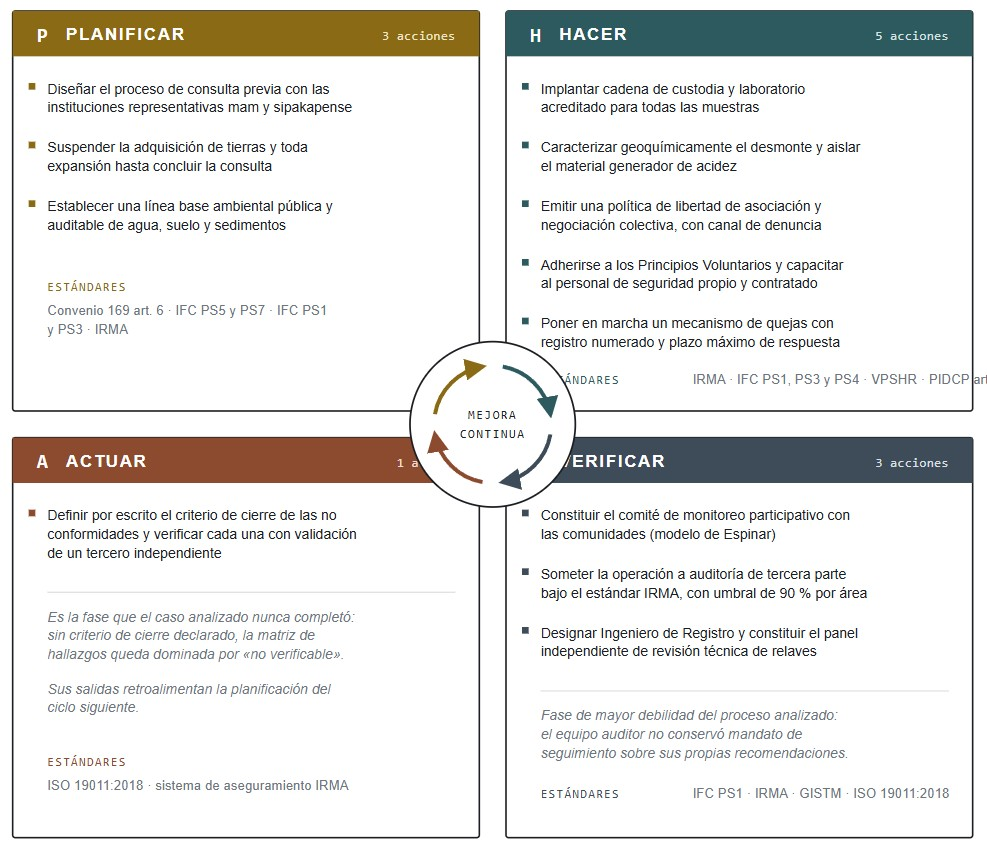
\includegraphics[width=0.8\textwidth]{imagenes/diagramas/ciclo_phva.pdf}
%  \caption{Ciclo PHVA aplicado a la gestión socioambiental de la Mina Marlin}
%  \label{fig:phva}
%  \footnotesize Nota. Elaboración propia a partir de \textcite{iso2015iso14001}.
%\end{figure}

\pendiente{desarrollar la sección 8 (6--8 páginas) + Tabla 4 + Figura 4}
       % Integrante 5
% =====================================================================
%  9. CONCLUSIONES
%  Responsable: INTEGRANTE 5
%  Extensión objetivo: 1,5 páginas — aprox. 550 palabras
%
%  DOS REGLAS QUE NO SE NEGOCIAN:
%   1. UNA CONCLUSIÓN POR CADA OBJETIVO ESPECÍFICO de la sección 2, en el
%      mismo orden. Si hay cinco objetivos, hay cinco conclusiones.
%   2. NO se introduce información nueva ni citas nuevas. Todo lo que se
%      concluye ya debe estar demostrado en las secciones 4 a 8.
% =====================================================================

\chapter{Conclusiones}

% TODO (conclusión 1 — responde al objetivo específico 1: describir la
%   unidad minera y su entorno):
%   La Mina Marlin fue una operación mixta de oro y plata sobre un depósito
%   epitermal de baja sulfuración, implantada en territorio de los pueblos
%   maya-mam y maya-sipakapense. Cierra señalando que la condición indígena
%   del territorio es el factor que determina todo el perfil de riesgo social.

% TODO (conclusión 2 — responde al objetivo 2: alcance, criterios y
%   metodología de la auditoría):
%   La HRIA fue una auditoría de desempeño en derechos humanos, no de
%   sistema de gestión, ejecutada por una firma independiente sobre criterios
%   internacionales y con alcance temporal y espacial declarados, incluidas
%   sus exclusiones.

% TODO (conclusión 3 — responde al objetivo 3: clasificar los hallazgos):
%   Indica cuántos hallazgos se clasificaron y en qué categorías, y cuál es
%   el eje más comprometido. Nombra el hallazgo de mayor gravedad (ausencia
%   de consulta previa) y por qué lo es.

% TODO (conclusión 4 — responde al objetivo 4: evaluar la independencia y
%   las limitaciones):
%   Toma posición argumentada sobre la tensión entre el financiamiento por
%   la empresa auditada y el diseño institucional que buscó mitigarlo, y
%   sobre el efecto del sesgo de participación en la validez de los hallazgos.

% TODO (conclusión 5 — responde al objetivo 5: proponer el plan PHVA):
%   Sintetiza qué aporta el plan propuesto y sobre qué estándares se apoya.

% TODO (conclusión de cierre, opcional pero recomendable):
%   Una reflexión final sobre la utilidad y los límites de la auditoría
%   socioambiental voluntaria como herramienta de control, y su relación con
%   la fiscalización estatal. Sin retórica: una idea, bien dicha.

\begin{enumerate}
  \item \pendiente{conclusión 1 — sobre la unidad minera}
  \item \pendiente{conclusión 2 — sobre el alcance y la metodología de la auditoría}
  \item \pendiente{conclusión 3 — sobre la clasificación de hallazgos}
  \item \pendiente{conclusión 4 — sobre la independencia y las limitaciones}
  \item \pendiente{conclusión 5 — sobre el plan de mejora continua}
\end{enumerate}
      % Integrante 5
% =====================================================================
%  10. RECOMENDACIONES
%  Responsable: INTEGRANTE 5
%  ESTADO: REDACTADO (1 de agosto de 2026) — ~800 palabras
%
%  DIFERENCIA CON LAS CONCLUSIONES: la conclusión mira hacia ATRÁS (qué se
%  encontró); la recomendación mira hacia ADELANTE (qué debe hacerse).
%  Cada recomendación tiene DESTINATARIO explícito: sin destinatario no es
%  una recomendación, es una opinión.
% =====================================================================

\section{Recomendaciones}
\label{sec:recomendaciones}

% ---------------------------------------------------------------------
\subsection{A la empresa operadora y al sector minero}

\begin{enumerate}
  \item \textbf{Establecer la línea base ambiental antes de operar, y hacerla
        pública.} Es la recomendación de mayor rendimiento de todo el informe y
        la de menor costo relativo. Una línea base pública, con puntos de muestreo
        acordados con las comunidades, protege tanto a la población frente a
        impactos no detectados como a la propia empresa frente a atribuciones
        infundadas. Su ausencia en este caso hizo que ninguna de las dos partes
        pudiera demostrar su posición.
  \item \textbf{Someterse a verificación independiente de tercera parte bajo un
        estándar auditable}, y no únicamente a autoevaluación o a evaluaciones de
        encargo. El estándar IRMA ofrece requisitos predefinidos, umbrales
        cuantificados y verificación periódica: los tres elementos que faltaron en
        el proceso analizado.
  \item \textbf{Definir por escrito el criterio de cierre de las no
        conformidades} y someterlo a validación de un tercero. Un plan de acción
        cuyo cumplimiento verifica quien debe cumplirlo no cierra el ciclo de
        mejora continua.
  \item \textbf{Adoptar formalmente los Principios Voluntarios en Seguridad y
        Derechos Humanos} y extender su aplicación a los contratistas de
        seguridad, con registro público de incidentes.
  \item \textbf{Sostener el monitoreo participativo y la transparencia de datos
        durante todo el post-cierre.} El empleo dura lo que dura la mina; el
        pasivo ambiental, no.
\end{enumerate}

% ---------------------------------------------------------------------
\subsection{Al Estado y a los organismos reguladores}

\begin{enumerate}
  \item \textbf{Garantizar la consulta previa, libre e informada antes del
        otorgamiento de la licencia}, no como respuesta al conflicto ya
        desatado. El caso demuestra que una consulta omitida no puede subsanarse
        después: solo puede repararse, que es un remedio inferior y más costoso
        para todas las partes.
  \item \textbf{Exigir línea base ambiental pública como requisito de la
        certificación ambiental}, con puntos de muestreo, parámetros y
        laboratorios acreditados definidos por la autoridad y no por el titular.
  \item \textbf{Dotar a la fiscalización ambiental de capacidad sancionadora
        efectiva y de recursos para ejercerla.} El contraste con el régimen
        peruano muestra que disponer del instrumento no equivale a usarlo con
        oportunidad; la experiencia de Espinar lo confirma.
  \item \textbf{Exigir el cumplimiento del Global Industry Standard on Tailings
        Management} en los depósitos de relaves, incluida la designación del
        Ingeniero de Registro y la constitución del panel independiente de
        revisión técnica.
  \item \textbf{Establecer garantías financieras de cierre suficientes y
        actualizables}, calculadas sobre el horizonte real del pasivo y no sobre
        el de la concesión.
\end{enumerate}

% ---------------------------------------------------------------------
\subsection{A las comunidades y organizaciones sociales}

\begin{enumerate}
  \item \textbf{Participar en los espacios de monitoreo ambiental participativo
        con capacitación técnica propia}, acceso a laboratorios acreditados y
        cadena de custodia documentada. El monitoreo comunitario gana o pierde
        credibilidad por su rigor metodológico, no por su origen: el modelo de
        Espinar es una referencia de escala útil.
  \item \textbf{Documentar y canalizar las quejas por los mecanismos formales},
        conservando registro propio de cada reclamo presentado y de la respuesta
        recibida. Ese registro es, con frecuencia, la única evidencia disponible
        cuando el caso escala a instancias externas.
  \item \textbf{Exigir la publicación de la línea base y de los resultados de
        monitoreo} como condición del diálogo, antes que como reclamo posterior.
\end{enumerate}

% ---------------------------------------------------------------------
\subsection{A la comunidad académica}

\begin{enumerate}
  \item \textbf{Desarrollar estudios epidemiológicos y de biomonitoreo de largo
        plazo con diseño acordado entre las partes}, capaces de distinguir el
        aporte geogénico del antropogénico. El conflicto de evidencia de este caso
        no se resolvió porque ningún estudio individual podía resolverlo con la
        metodología disponible.
  \item \textbf{Investigar comparativamente la eficacia de la auditoría
        voluntaria frente a la fiscalización estatal} en contextos de
        conflictividad socioambiental minera en América Latina, midiendo cambio
        efectivo de conducta y no solo emisión de recomendaciones.
  \item \textbf{Documentar los procesos de post-cierre minero}, que constituyen
        la fase menos estudiada y la de mayor horizonte temporal.
\end{enumerate}
   % Integrante 5

% ------------------------------------------------------------
%  REFERENCIAS
%  Estilo IEEE numérico: las citas salen como [1], [2], ordenadas
%  por orden de aparición en el texto.
%
%  \nocite{*} fuerza que TODAS las entradas de referencias.bib
%  aparezcan aunque aún no estén citadas. Es útil mientras se redacta.
%  >>> COMENTAR ESTA LÍNEA ANTES DE LA ENTREGA FINAL <<<
% ------------------------------------------------------------
\nocite{*}
\printbibliography[heading=referencias,title={Referencias}]

% ------------------------------------------------------------
%  ANEXOS
%  Vuelven a UNA columna: las matrices de no conformidades y la
%  cronología usan longtable, que no funciona en dos columnas.
% ------------------------------------------------------------
\onecolumn
% =====================================================================
%  ANEXOS
%  Responsables: INTEGRANTE 2 (Anexos A y E) e INTEGRANTE 4 (Anexos B, C y D)
%  Extensión: libre, no cuenta para el objetivo de páginas del cuerpo.
%
%  DOS COSAS IMPORTANTES DE ESTE FORMATO:
%
%  1. main.tex conmuta a UNA COLUMNA (\onecolumn) antes de incluir este
%     archivo. Por eso aquí SÍ se puede usar longtable, que no funciona
%     en modo de dos columnas. Es el único sitio del informe donde se
%     puede.
%
%  2. Los anexos se rotulan a mano (Anexo A, B, C...) con \chapter* y se
%     añaden al índice con \addcontentsline. No se usa \appendix: en
%     IEEEtran, combinado con el adaptador de jerarquía del preámbulo,
%     produce resultados impredecibles.
% =====================================================================

\newpage
\chapter*{Anexo A. Mapa de ubicación ampliado}
\addcontentsline{toc}{section}{Anexo A. Mapa de ubicación ampliado}
\label{anexo:mapa}

% TODO: Versión a página completa del mapa de la Figura 1, con el detalle de
%   los municipios de San Miguel Ixtahuacán y Sipacapa, las cuencas de los
%   ríos Tzalá, Quivichil y Cuilco, y la ubicación de la planta y del
%   depósito de relaves.
%   RECORDATORIO DE LICENCIA: si el mapa base es de OpenStreetMap, la
%   atribución «© OpenStreetMap contributors» (licencia ODbL) es obligatoria.
%   Si usas el mapa del conflicto de OCMAL, cítalo. \cite{ocmalsfmarlin}
%
%\begin{figure}
%  \centering
%  \includegraphics[width=0.9\textwidth]{imagenes/mapas/mapa_ampliado.png}
%  \caption{Mapa ampliado del área de influencia de la Mina Marlin}
%  \label{fig:mapa-ampliado}
%\end{figure}

\newpage
\chapter*{Anexo B. Matriz de no conformidades completa}
\addcontentsline{toc}{section}{Anexo B. Matriz de no conformidades completa}
\label{anexo:matriz}

% TODO: En el capítulo 6 va un EXTRACTO de la matriz (los hallazgos
%   principales, en una tabla que abarca las dos columnas). Aquí va la
%   matriz ÍNTEGRA, con todos los hallazgos de los siete ejes.
%   Como estamos a una columna, aquí sí funciona longtable.
%
%\begin{landscape}
%\begin{footnotesize}
%\begin{longtable}{@{}L{1.8cm} L{4cm} L{4cm} L{3cm} L{1.8cm} L{4cm} L{2cm}@{}}
%  \caption{Matriz completa de no conformidades de la auditoría socioambiental de la Mina Marlin}
%  \label{tab:matriz-nc-completa} \\
%  \toprule
%  \textbf{Eje} & \textbf{Hallazgo} & \textbf{Evidencia objetiva} & \textbf{Criterio incumplido} & \textbf{Clasif.} & \textbf{Recomendación} & \textbf{Estado de cierre} \\
%  \midrule
%  \endfirsthead
%  \multicolumn{7}{l}{\footnotesize\textit{Tabla \ref{tab:matriz-nc-completa} (continuación)}} \\
%  \toprule
%  \textbf{Eje} & \textbf{Hallazgo} & \textbf{Evidencia objetiva} & \textbf{Criterio incumplido} & \textbf{Clasif.} & \textbf{Recomendación} & \textbf{Estado de cierre} \\
%  \midrule
%  \endhead
%  \bottomrule
%  \multicolumn{7}{l}{\footnotesize Fuente: elaboración propia a partir de \cite{oncommonground2010hria}.} \\
%  \endlastfoot
%  Consulta    & & & Convenio 169 {OIT}, art. 6 & \NCmayor & & \\
%  Ambiente    & & &                            &          & & \\
%  Trabajo     & & &                            &          & & \\
%  Tierras     & & & {IFC} {PS}5                &          & & \\
%  Inversión   & & &                            &          & & \\
%  Seguridad   & & & {VPSHR}                    &          & & \\
%  Remediación & & & {IFC} {PS}1                &          & & \\
%\end{longtable}
%\end{footnotesize}
%\end{landscape}

\newpage
\chapter*{Anexo C. Cronología del caso (1996--2017)}
\addcontentsline{toc}{section}{Anexo C. Cronología del caso (1996--2017)}
\label{anexo:cronologia}

% TODO: Tabla de dos columnas (fecha / hecho). Hitos que no pueden faltar:
%   06/08/1996  Constitución de Montana Exploradora de Guatemala, S.A.
%   1998        Descubrimiento del yacimiento.
%   2000        Adquisición por Francisco Gold.
%   2002        Fusión con Glamis Gold.
%   2003        Préstamo de la IFC por US$ 45 millones.
%   27/11/2003  Licencia de explotación del Ministerio de Energía y Minas.
%   2004-2005   Construcción de la mina.
%   2004        Revisión independiente del EIA por Robert Moran.
%   2005        Consulta comunitaria de Sipacapa; queja de Madre Selva ante la CAO.
%   Fines 2005  Inicio de producción.
%   05/2006     Cierre del caso CAO Marlin-01/Sipacapa.
%   2006        Goldcorp adquiere Glamis Gold.
%   03/2008     Firma del MOU para la evaluación de derechos humanos.
%   10/2008     Selección de On Common Ground Consultants.
%   05/2010     Publicación de la HRIA.
%   20/05/2010  La CIDH otorga medidas cautelares MC 260-07.
%   2010        Estudio de salud de Physicians for Human Rights / U. de Michigan.
%   2010        Pronunciamiento de la CEACR de la OIT.
%   12/2011     La CIDH modifica las medidas cautelares.
%   2013        Instalación de la planta de relaves filtrados (dry-stack).
%   31/05/2017  Cierre de producción de la mina.
%
%\begin{longtable}{@{}L{3cm} L{12cm}@{}}
%  \caption{Cronología del caso Mina Marlin} \label{tab:cronologia} \\
%  \toprule \textbf{Fecha} & \textbf{Hecho} \\ \midrule \endfirsthead
%  \toprule \textbf{Fecha} & \textbf{Hecho} \\ \midrule \endhead
%  \bottomrule \endlastfoot
%   & \\
%\end{longtable}

\newpage
\chapter*{Anexo D. Fichas de los estándares aplicados}
\addcontentsline{toc}{section}{Anexo D. Fichas de los estándares aplicados}
\label{anexo:estandares}

% TODO: Una ficha breve por estándar, con: nombre completo, organismo emisor,
%   año, carácter (obligatorio / voluntario / certificable), alcance y
%   pertinencia para este caso. Estándares a fichar:
%   ISO 14001:2015, ISO 19011:2018, IFC Performance Standards,
%   Convenio 169 de la OIT, VPSHR, ICMM Mining Principles, GISTM e IRMA.
%   Sugerencia: la macro \recuadro{título}{contenido} del preámbulo da un
%   formato de ficha limpio y homogéneo.

\newpage
\chapter*{Anexo E. Glosario de siglas}
\addcontentsline{toc}{section}{Anexo E. Glosario de siglas}
\label{anexo:glosario}

% TODO: Lista alfabética. Como mínimo:
%   AMAC    Asociación de Monitoreo Ambiental Comunitario
%   ARD     Drenaje ácido de roca (acid rock drainage)
%   CAO     Compliance Advisor Ombudsman
%   CEACR   Comisión de Expertos en Aplicación de Convenios y Recomendaciones (OIT)
%   CIDH    Comisión Interamericana de Derechos Humanos
%   CIL     Carbon in leach (lixiviación con carbón en pulpa)
%   COPAE   Comisión Pastoral Paz y Ecología
%   DIHR    Danish Institute for Human Rights
%   EIA     Estudio de impacto ambiental
%   GISTM   Global Industry Standard on Tailings Management
%   HRCA    Human Rights Compliance Assessment
%   HRIA    Human Rights Impact Assessment
%   ICMM    International Council on Mining and Metals
%   IFC     International Finance Corporation
%   IRMA    Initiative for Responsible Mining Assurance
%   MOU     Memorando de entendimiento
%   NC      No conformidad
%   OCMAL   Observatorio de Conflictos Mineros de América Latina
%   OEFA    Organismo de Evaluación y Fiscalización Ambiental (Perú)
%   OIT     Organización Internacional del Trabajo
%   PAMA    Programa de adecuación y manejo ambiental
%   PHVA    Planificar, Hacer, Verificar, Actuar
%   PS      Performance Standard (IFC)
%   SEIA    Sistema Nacional de Evaluación de Impacto Ambiental
%   SGA     Sistema de gestión ambiental
%   TSF     Tailings storage facility (depósito de relaves)
%   VPSHR   Voluntary Principles on Security and Human Rights

\pendiente{completar los anexos A a E}
            % Integrantes 2 y 4

\end{document}
